% file thesis.tex
% Archivo thesis.tex
% Documento maestro que incluye todos los paquetes necesarios para el documento
% principal.

% Documento obtenido por un sinfin de iteraciones de administradores del LDC
% Estructura actual hecha por:
% Jairo Lopez <jairo@ldc.usb.ve>
% Actualizado ligeramente por:
% Alexander Tough 

\documentclass[oneside,12pt,letterpaper]{report}
\tolerance=1000  
\hbadness=10000  
\raggedbottom

% Macros personalizados
\newcommand{\entry}{\textit{entry}}
\newcommand{\entries}{\textit{entries}}
\newcommand{\activity}{\textit{activity}}

% Para escribir algoritmos
\usepackage{listings}
\usepackage{algpseudocode}
\usepackage{algorithmicx}
\usepackage{algorithm}

\usepackage{pdflscape}

% Paquetes para manejar graficos
\usepackage{epsf}
\usepackage[pdftex]{graphicx}
\usepackage{epsfig}
% Simbolos matematicos
\usepackage{latexsym,amssymb}
% Paquetes para presentar una tesis decente.
\usepackage{setspace,cite} % Doble espacio para texto, espacio singular para
                           % los caption y pie de pagina

\usepackage[table]{xcolor}
\usepackage{tikz}
\usetikzlibrary{shapes.geometric,arrows}

\usetikzlibrary{arrows,shapes}
\usepackage{verbatim}

\usepackage{comment}

% Paquetes no utilizados para citas
%\usepackage{mcite} 
%\usepackage{draft} 

\usepackage{wrapfig}
\usepackage{alltt}

% Acentos 
\usepackage[spanish,activeacute,es-noquoting]{babel}

\usepackage[spanish]{translator}
\usepackage[utf8]{inputenc}
\usepackage{color, xcolor, colortbl}
\usepackage{multirow}
\usepackage{subfig}
\usepackage[OT1]{fontenc}
\usepackage{tocbibind}
\usepackage{anysize}
\usepackage{listings} 

% Para poder tener texto asiatico
%\usepackage{CJK}

\usepackage{pdfpages}

% Opciones para los glosarios
\usepackage[style=altlist,toc,numberline,acronym]{glossaries}
\usepackage{url}
\usepackage{amsthm}
\usepackage{amsmath}
\usepackage{fancyhdr} % Necesario para los encabezados
\usepackage{fancyvrb}
\usepackage{makeidx} % En caso de necesitar indices.
\makeindex  % Necesitado para los indices

% Definiciones para definicions, teoremas y lemas
\theoremstyle{definition} \newtheorem{definicion}{Definici\'{o}n}
\theoremstyle{plain} \newtheorem{teorema}{Teorema}
\theoremstyle{plain} \newtheorem{lema}{Lema}

% Para la creacion de los pdfs
\usepackage{hyperref}

% Para resolver el lio del Unicode para la informacion de los PDFs
% En pdftitle coloca el nombre de su proyecto de grado/pasantia.
% En pdfauthor coloca su nombre.
\hypersetup{
    pdftitle = {Desarrollo de una aplicación móvil de control y reportes de gastos},
    pdfauthor={Susana Charara Charara},
    colorlinks,
    citecolor=black,
    filecolor=black,
    linkcolor=black,
    urlcolor=black,
    backref,
    pdftex
}

\definecolor{brown}{rgb}{0.7,0.2,0}
\definecolor{darkgreen}{rgb}{0,0.6,0.1}
\definecolor{darkgrey}{rgb}{0.4,0.4,0.4}
\definecolor{lightgrey}{rgb}{0.95,0.95,0.95}

\usepackage{listings}
\lstnewenvironment{code}{\lstset{basicstyle=\small}}{}

\lstset{escapeinside=~~}
\lstset{
   frame=single,
   framerule=1pt,
   showstringspaces=false,
   basicstyle=\footnotesize\ttfamily,
   keywordstyle=\textbf,
   backgroundcolor=\color{lightgrey}
}

% Crea el glosario
\makeglossaries

% Incluye el glosario
\newglossaryentry{PILA}
{
  name=Pila,
  description={Es una lista en la que el modo de agregar sus elementos es de tipo 
	último en entrar, primero en salir que permite almacenar y recuperar datos.}
}

\newglossaryentry{COLA}
{
  name=Cola,
  description={Es una lista en la que el modo de agregar sus elementos es de tipo 
	primero en entrar, primero en salir que permite almacenar y recuperar datos.}
}

\newglossaryentry{ARREGLO}
{
  name=Arreglo,
  description={Es una lista ordinal en la que el modo de acceso a sus elementos 
  es indexado que permite almacenar y recuperar datos pero no modificar su
  tamaño inicial.}
}

\newglossaryentry{GRAFO}
{
  name=Grafo,
  description={Es una red que une nodos que permiten almacenar y recuperar datos.}
}


% Para crear la hoja escaneada de las firmas
\usepackage[absolute]{textpos}

% Pone los nombres y las opciones para mostrar los codigos fuentes
\lstset{language=C, breaklines=true, frame=single, showstringspaces=false,
        showtabs=false, numbers=left, keywordstyle=\color{black},
        basicstyle=\footnotesize, captionpos=b }
\renewcommand{\lstlistingname}{C\'{o}digo fuente}
\renewcommand{\lstlistlistingname}{\'{I}ndice de c\'{o}digos fuentes}

\newcommand{\todo}{ TODO: }

% Dimensiones de la pagina
\setlength{\headheight}{15pt}
\marginsize{3cm}{2cm}{2cm}{2cm}

%%%%%%%%%%%%%%%%%%%%%%%%%%%%%%%%%%%%%%%%%%%%%%%%%%%%%%%%%%%%%%%%%%%%%%%%%%%
%%%%%%%%%%%%%%%%      end of preamble and start of document     %%%%%%%%%%%
%%%%%%%%%%%%%%%%%%%%%%%%%%%%%%%%%%%%%%%%%%%%%%%%%%%%%%%%%%%%%%%%%%%%%%%%%%%
\begin{document}

% Pagina de titulo
% Pagina de titulo
\begin{titlepage}
\begin{center}

% Upper part (aqui ya esta incluido el logo de la USB).

\includegraphics[scale=0.5,type=png,ext=.png,read=.png]{imagenes/cebolla} \\

% Encabezado
\textsc {\large UNIVERSIDAD SIMÓN BOLÍVAR} \\
\textsc{\bfseries DECANATO DE ESTUDIOS PROFESIONALES\\
COORDINACI'ON DE INGENIER'IA DE LA COMPUTACI'ON}

\bigskip
\bigskip
\bigskip
\bigskip
\bigskip
\bigskip
\bigskip
\bigskip
\bigskip

% Title/Titulo
% Aqui ponga el nombre de su proyecto de grado/pasantia larga
\textsc{\bfseries DESARROLLO DE UNA APLICACIÓN MÓVIL DE CONTROL Y REPORTES DE GASTOS}

\bigskip
\bigskip
\bigskip
\bigskip
\bigskip

% Author and supervisor/Autor y tutor
\begin{minipage}{\textwidth}
\centering
Por: \\ SUSANA CHARARA CHARARA \\

\bigskip
\bigskip
\bigskip

Realizado con la asesoría de: \\
Tutor Académico: XIOMARA CONTRERAS \\
Tutor Industrial: LUIS AUGUSTO PEÑA PEREIRA
\end{minipage}

\bigskip
\bigskip
\bigskip
\bigskip
\bigskip
\bigskip
\bigskip
\bigskip
\bigskip

% Bottom half
{INFORME DE PASANTÍA LARGA \\ Presentado ante la Ilustre Universidad Simón Bolívar \\
como requisito parcial para optar al título de \\ Ingeniero en Computación} \\

\bigskip
\bigskip
\vfill

% Date/Fecha 
{\large \bfseries Sartenejas, 
%FECHA
SEPTIEMBRE de 2016}

\end{center}
\end{titlepage}

% Pagina de titulo
\begin{titlepage}
\begin{center}

% Upper part (aqui ya esta incluido el logo de la USB).

\includegraphics[scale=0.5,type=png,ext=.png,read=.png]{imagenes/cebolla} \\

% Encabezado
\textsc {\large UNIVERSIDAD SIMÓN BOLÍVAR} \\
\textsc{\bfseries DECANATO DE ESTUDIOS PROFESIONALES\\
COORDINACI'ON DE INGENIER'IA DE LA COMPUTACI'ON}

\bigskip
\bigskip
\bigskip
\bigskip
\bigskip
\bigskip
\bigskip
\bigskip
\bigskip

% Title/Titulo
% Aqui ponga el nombre de su proyecto de grado/pasantia larga
\textsc{\bfseries DESARROLLO DE UNA APLICACIÓN MÓVIL DE CONTROL Y REPORTES DE GASTOS}

\bigskip
\bigskip
\bigskip
\bigskip
\bigskip

% Author and supervisor/Autor y tutor
\begin{minipage}{\textwidth}
\centering
Por: \\ SUSANA CHARARA CHARARA \\

\bigskip
\bigskip
\bigskip

Realizado con la asesoría de: \\
Tutor Académico: XIOMARA CONTRERAS \\
Tutor Industrial: LUIS AUGUSTO PEÑA PEREIRA
\end{minipage}

\bigskip
\bigskip
\bigskip
\bigskip
\bigskip
\bigskip
\bigskip
\bigskip
\bigskip

% Bottom half
{INFORME DE PASANTÍA LARGA \\ Presentado ante la Ilustre Universidad Simón Bolívar \\
como requisito parcial para optar al título de \\ Ingeniero en Computación} \\

\bigskip
\bigskip
\vfill

% Date/Fecha 
{\large \bfseries Sartenejas, 
%FECHA
SEPTIEMBRE de 2016}

\end{center}
\end{titlepage}

% Pagina de acta final (vacio)
%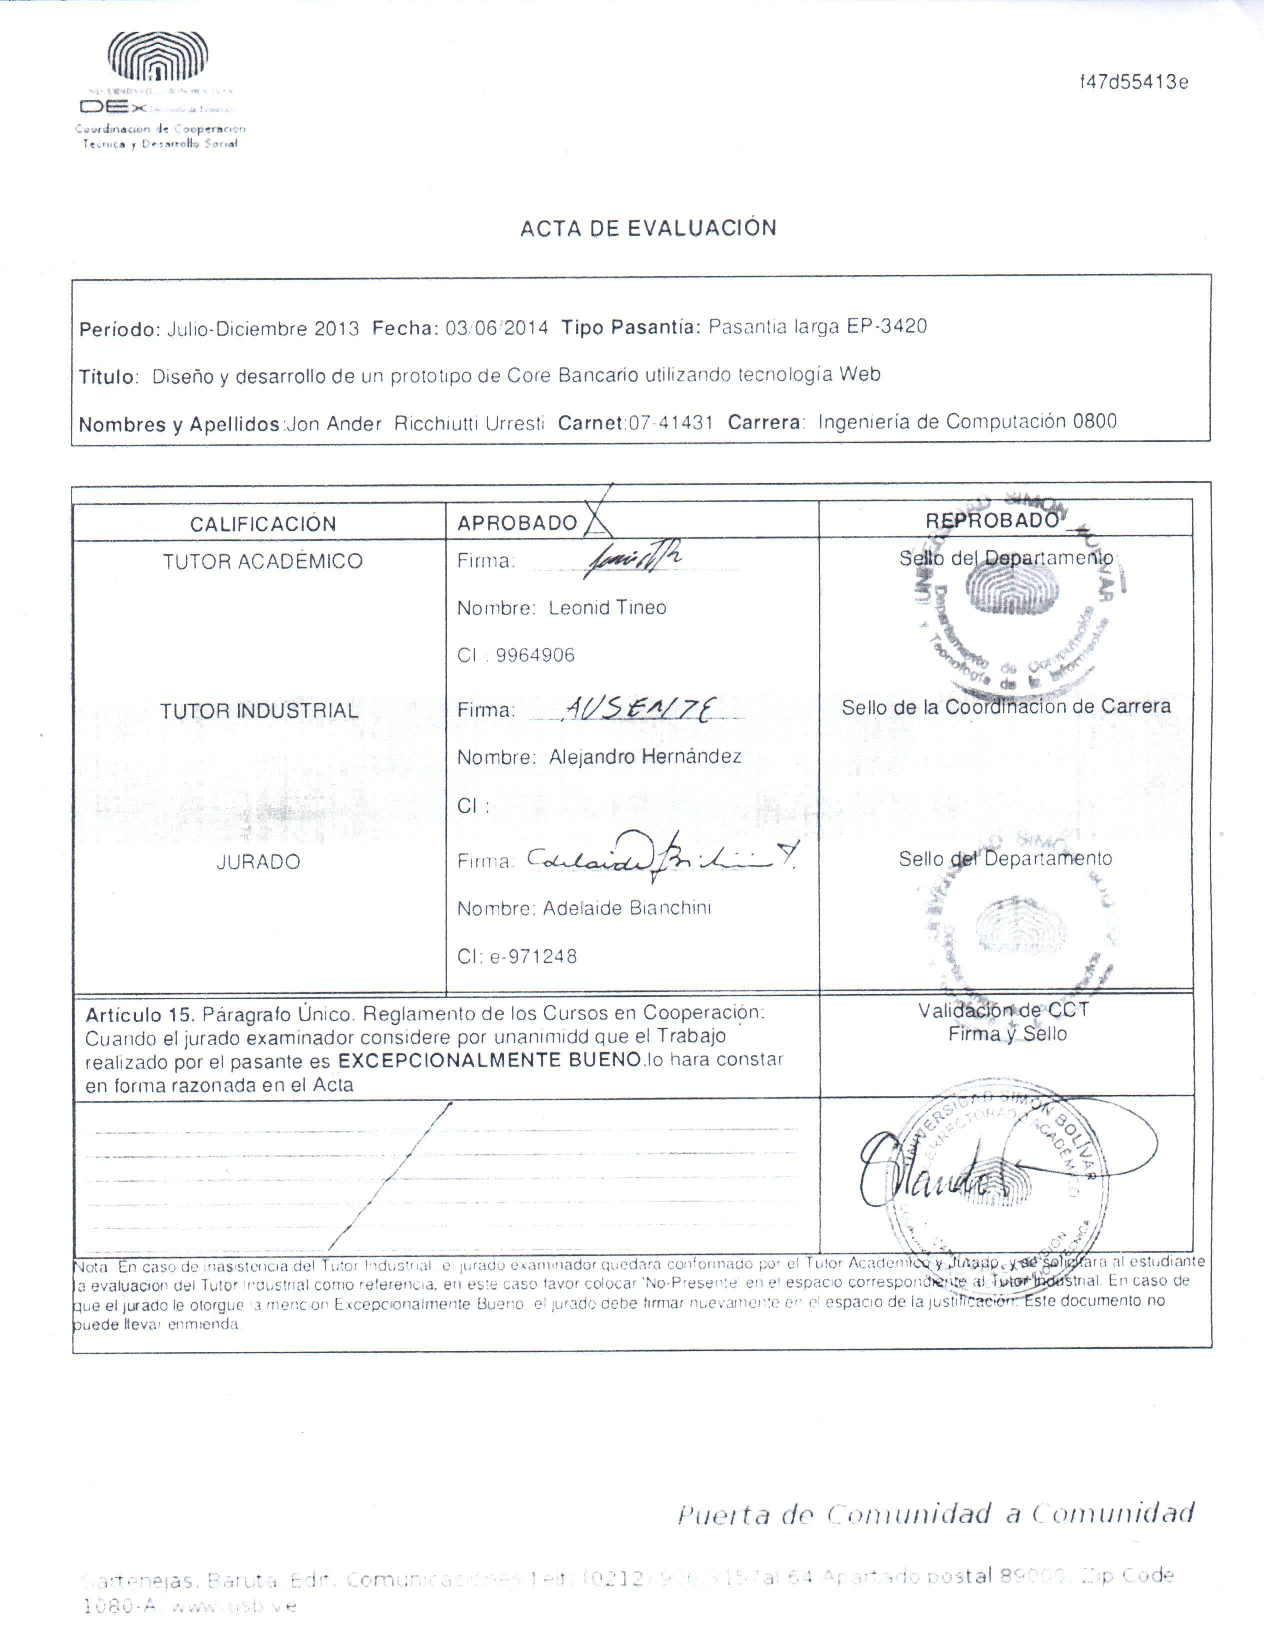
\includepdf[pages={1}]{intro/firmas.pdf}

\setcounter{secnumdepth}{4}
\setcounter{tocdepth}{5}

% Define encabezado numeros romanos y como se separan los captiulos y las
% secciones
\addtolength{\headheight}{3pt}
\pagenumbering{roman}
\pagestyle{fancyplain}

\renewcommand{\chaptermark}[1]{\markboth{\chaptername\ \thechapter:\,\ #1}{}}
\renewcommand{\sectionmark}[1]{\markright{\thesection\,\ #1}}

\onehalfspacing

\lhead{}
\chead{}
\rhead{}
\renewcommand{\headrulewidth}{0.0pt}
\lfoot{}
\cfoot{\fancyplain{}{\thepage}}
\rfoot{}


% Pagina de resumen
\setcounter{page}{3}
\begin{center}
	{\bf Resumen} \pdfbookmark[0]{Resumen}{resumen} % Sets a PDF bookmark for the dedication
\end{center}	

En esta pasantía se desarrolló, para la empresa Digitalica Group, C.A., una aplicación para dispositivos móviles con la cual se pueden realizar reportes de gastos. Actualmente, la empresa Digitalica Group, C.A. ofrece a sus trabajadores el beneficio de realizar reembolsos de gastos en ciertos rubros; el proyecto nació como solución al problema de agilizar el proceso en que los trabajadores hacen llegar a los supervisores la información de estos gastos. Con la aplicación desarrollada, se pueden registrar gastos e ingresos con un monto, fecha y descripción. Se permite también capturar y guardar fotos tanto de los ingresos como de los gastos, de manera que el usuario puede tomar fotos de los recibos de sus gastos. Además, estos gastos/ingresos pueden estar asociados a categorías, que indican el rubro al que pertenecen. La aplicación permite al usuario generar archivos con formato PDF que contienen un reporte con una lista de gastos, en un rango de fecha determinado; estos reportes se pueden enviar a un servidor web. Este servidor también fue desarrollado durante la pasantía; con él, se prestan los servicios necesarios para que la aplicación pueda autenticar usuarios y enviar reportes. Igualmente, se desarrolló una aplicación web que permite a los supervisores de la empresa revisar los reportes recibidos, aprobarlos y rechazarlos.

En este informe se describen los conceptos teóricos que ayudaron al diseño y desarrollo de la solución. Igualmente, se describe el proceso de desarrollo de los tres componentes principales desarrollados durante la pasantía: aplicación nativa para Android, servidor web y aplicación web. El desarrollo de estos involucró el diseño e implementación de los modelos de datos de la aplicación y el servidor, así como múltiples interfaces de usuario que permiten la interacción con los modelos. Para cada componente, se describen el entorno de trabajo y las herramientas utilizadas. Se utilizó Java como lenguaje de programación tanto de la aplicación móvil como del servidor; entre las herramientas que se emplearon en el desarrollo del servidor se pueden mencionar AppFuse, Spring, Hibernate y Tapestry, entre otros.

Por otra parte, se utilizó Scrum como marco de trabajo, dividiendo el desarrollo del proyecto en ocho iteraciones, en las que se implementaron los componentes y funcionalidades necesarios para el cumplimiento de los objetivos de la pasantía.

El objetivo del desarrollo de la pasantía fue ofrecer una solución al problema que actualmente se presenta en la empresa de agilizar el proceso de reembolso sobre ciertos gastos.




% Pagina de dedicatoria (opcional)
%\pagebreak

%\setcounter{page}{5}

\vspace*{8cm} 
\pdfbookmark[0]{Dedicatoria}{dedicatoria} % Sets a PDF bookmark for the dedication
\begin{center} 
\large A nuestros padres.\\ Porque nos dieron la vida y nos han guiado 
a ser quienes somos hoy.
\end{center}
\newpage


% Pagina de agradecimientos (opcional)
%%\setcounter{page}{6}

\chapter*{Agradecimientos
\markboth{Agradecimientos}{Agradecimientos}}
\pdfbookmark[0]{Agradecimientos}{agradecimientos}

\bigskip



% Crea la tabla de contenidos
\tableofcontents

% Crea la lista de cuadros
\listoftables

% Crea la lista de figuras
\listoffigures
%\newpage
\phantomsection
%\setcounter{page}{4}
\chapter*{Lista de Símbolos y Abreviaturas}% Sets a PDF bookmark for the dedication

\vspace{5 mm}
\noindent
\textbf{BPM:} Business Process Management (en español Gestión de Procesos de Negocio)\\ \\

\addcontentsline{toc}{chapter}{Lista de Símbolos y Abreviaturas}

% Crea la lista de codigos fuentes
%\lstlistoflistings

\clearpage

% Define encabezado en numeros arabicos  
\pagenumbering{arabic}

\fancyhf{} % Redefine el encabezado 
\lhead{}
\chead{}
\rhead{\fancyplain{}{\thepage}}
\renewcommand{\headrulewidth}{0.0pt}
\lfoot{}
\cfoot{}
\rfoot{}

\doublespacing

% Incluye los archivos deseados - El contenido de su proyecto de grado/pasantia larga.
\phantomsection
\addcontentsline{toc}{chapter}{Introducción}
\chapter*{Introducción} \label{sec:Introduccion}
%\pdfbookmark[0]{Introducción}{introduccion} % Sets a PDF bookmark for the dedication

\vspace{5 mm}
En la actualidad, empresas como Digitalica Group, C.A., le ofrecen a sus empleados el beneficio de realizar cierta cantidad de gastos mensuales y posteriormente iniciar un proceso de reembolso. Este proceso puede tomar mucho tiempo y puede resultar difícil si se hace manualmente, pues implica que el trabajador debe guardar todas las facturas de los gastos implicados durante el mes; al finalizar el mes debe entregar las facturas a la empresa y esta última inicia un proceso de verificación para culminar con el proceso de reembolso. Igualmente, para que la empresa pueda mantener un control y registro de todos los gastos que han sido reembolsados, debe guardar todos los meses las facturas de todos sus trabajadores, para lo que es necesario contar con un espacio físico que lo permita. 

Dado que Digitalica Group, C.A. es una empresa dedicada al desarrollo de \textit{software}, decidió automatizar todo el proceso de reembolso, mediante la creación de una aplicación móvil\footnote{Para efectos de simplicidad, se utilizará a lo largo del libro el término \textit{aplicación móvil} para hacer referencia a aplicaciones que se ejecutan en dispositivos móviles.} y un servidor. De esta manera, con la aplicación los trabajadores pueden mantener un registro de gastos dentro de un dispositivo móvil, y con el servidor web se mantiene organizada y centralizada la información de estos gastos.
%Dada la necesidad de agilizar el proceso de reembolso, la empresa Digitalica Group, C.A. decidió crear una aplicación móvil\footnote{Para efectos de simplicidad, se utilizará a lo largo del libro el término \textit{aplicación móvil} para hacer referencia a aplicaciones que se ejecutan en dispositivos móviles.} que permita a sus trabajadores mantener un registro de gastos dentro de un dispositivo móvil.

%Actualmente existen aplicaciones móviles que sirven para llevar un registro de gastos. Sin embargo, estas aplicaciones no satisfacen las necesidades de Digitalica Group, C.A. por diversas razones:

%\begin{itemize}

%\item La empresa realiza el reembolso de gastos en ciertos rubros y para esto se debe especificar a qué categoría pertenece cada gasto. Las aplicaciones ya existentes pueden limitar el proceso al no contar con la posibilidad de poder asociar un gasto a un rubro cubierto por la empresa.

%\item Se desea crear archivos de reportes de los gastos registrados por los trabajadores. Se desea que estos reportes puedan ser personalizados y presenten una estructura particular.
%\item Se desea mantener centralizada toda la información referente a estos reportes, de manera que se pueda acceder a la misma de una manera más fácil.
%\item Si el proceso de reembolso sufre alguna modificación, se desea contar con una aplicación que tome en cuenta los nuevos cambios.
%\end{itemize}

Esta aplicación debe contar con las siguientes funcionalidades:

\begin{itemize}
\item Registrar gastos con su fecha, monto, una breve descripción, fotos y categoría a la que pertenecen.
\item Organizar y consultar gastos con criterios de búsqueda pre-establecidos.
\item Crear reportes personalizados con los gastos y enviar dichos reportes a un servidor.
\item Enviar reportes mediante archivos con formato PDF a los supervisores.
\end{itemize}

En cuanto al servidor, éste debe proveer funcionalidades que permitan controlar el estado de aprobación de los reportes recibidos.

En este informe se describe el proceso de desarrollo de una aplicación móvil y de un servidor web que cumplen con los requisitos mencionados anteriormente.

El informe se estructura de la siguiente manera: En el Capítulo~\ref{chap:Entorno Empresarial} se describe de una forma general la empresa; en el Capítulo~\ref{chap:Marco Teorico} se definen los conceptos teóricos estudiados para el desarrollo del proyecto; en el Capítulo~\ref{chap:Marco Tecnologico} se mencionan las herramientas y tecnologías que facilitaron el desarrollo; en el Capítulo~\ref{chap:Marco Metodologico} se describe brevemente el marco de trabajo utilizado, Scrum; en el Capítulo~\ref{chapter:Desarrollo de la aplicacion} se describen todas las fases involucradas tanto en el diseño como el desarrollo de la solución; en el Capítulo~\ref{chap:conclusiones} se exponen las conclusiones y recomendaciones que surgieron luego de la investigación y desarrollo del proyecto; finalmente, se muestran las referencias bibliográficas consultadas.
%
% Entorno empresarial.
\chapter{Entorno Empresarial} \label{chap:Entorno Empresarial}

\vspace{5 mm}

\section{Descripción de la empresa} \label{Descripcion de la empresa}

Digitalica Group, C.A. es una empresa que se dedica al desarrollo de soluciones móviles, aplicaciones empresariales y \textit{middleware}. Se caracteriza por estar a la vanguardia, utilizando tecnologías innovadoras\cite{DIG1}. Sus principales servicios son:

\begin{itemize}
\item Consultoría en el área de desarrollo de aplicaciones móviles: Durante los últimos años se ha brindado apoyo en el área de soluciones móviles a empresas del sector educativo.
\item Desarrollo de \textit{software} y aplicaciones móviles para clientes. Se han desarrollado aplicaciones para medios de comunicación nacionales e internacionales, así como para empresas del sector educativo.
\item Ofrecer \textit{software} como un servicio: Actualmente, los productos que ofrece la empresa están enfocados en el área de noticias, medios de comunicación y registro de gastos e ingresos. 
\end{itemize}

\section{Misión} \label{Mision}

"Proveer soluciones y servicios de consultoría basados en tecnolías móviles, utilizando la mejores herramientas, metodologías y estándares de calidad en la industria" \cite{DIG1}.
\section{Visión} \label{Vision}
"Ser el líder en Latinoamérica en brindar soluciones innovadoras basadas en tecnologías móviles, con un equipo creativo con los conocimientos más sólidos en tecnologías de información para móviles, para cometir en el mercado global" \cite{DIG1}.
\section{Estructura organizacional} \label{Estuctura organizacional}

La estructura organizacional de la empresa está comprendida principalmente por la Junta de Directores, como se muestra en la figura 1.1.

\begin{figure}[ht]
  \centering
  \includegraphics[scale=0.45,type=png,ext=.png,read=.png]{imagenes/estructura_empresa}
  \caption{Estructura organizacional de la empresa}
  \label{fig:estructuraEmpresa}
\end{figure}

La Junta de Directores está compuesta por tres cargos: Director de Operaciones (COO por sus siglas en inglés), Director Ejecutivo (CEO por sus siglas en inglés) y Director de Tecnología (CTO por sus siglas en inglés).

El COO se encarga de gestionar las adquisiciones de la empresa y de mantener la infraestructura tecnológica.

El CEO se encarga de manejar la Dirección de Ventas, dirigir el Departamento Legal junto al abogado y dirigir el Departamento de Finanzas y Recursos Humanos junto al contador.

El CTO se encarga de dirigir el departamento de desarrollo,por lo que el equipo de desarrollo de \textit{software} se comunica y le rinde cuentas a él.



\section{Ubicación del pasante} \label{Ubicacion del pasante}

Los pasantes se encuentran en el Departamento de Desarrollo, dirigido por el CTO, y donde se encuentan los especialistas de todas las áreas de desarrollo de \textit{software}. Esto permite que los pasantes estén en constante contacto con personas que puedan asistirlos y solventar las dudas que puedan surgir durante el desarrollo.



 % Marco Teorico.
\chapter{Marco Teórico} \label{chap:Marco Teorico}

En este capítulo se exponen los conceptos teóricos estudiados, tanto para entender las tecnologías utilizadas como para realizar el desarrollo de \textit{software} requerido. Los conceptos estudiados formaron parte fundamental del proceso de diseño y desarrollo de la solución.

\section{Patrones de diseño} \label{sect:Patrones de diseno}

Un patrón de diseño es una solución general y repetible a problemas que suelen presentarse en el proceso de diseño de software. Para que una solución pueda ser considerada como un patrón de diseño debe ser reutilizable, es decir, que se pueda aplicar a diferentes problemas de diseño en diferentes situaciones \cite{DSP0}. A continuación se describen los patrones utilizados en el diseño de la solución del proyecto.


\subsection{\textit{Singleton}}

El \textit{singleton} es un patrón de diseño que asegura la existencia de una sola instancia de la clase que lo implementa \cite{DSP1}. Esto es útil cuando se necesita únicamente un objeto para coordinar las acciones en el sistema \cite{SNG0}.

\subsection{\textit{Adapter}}

Transforma la interfaz de una clase en otra interfaz que el cliente espera. Esto permite que una clase que no pueda utilizar la primera interfaz, sí pueda hacerlo a través de la otra \cite{DSP1}.

\subsection{\textit{Facade}}

Se utiliza para ofrecer una interfaz sencilla para operaciones complejas. Con este patrón se logra ofrecer una interfaz de alto nivel que hace que el sistema sea más fácil de usar para los clientes \cite{DSP1}.
%\subsection{\textit{Factory}} 


\section{Patrones de arquitectura} \label{sect:Patrones de arquitectura}
Un patrón de arquitectura es una solución a problemas de arquitectura de \textit{software}, ayudando a definir una estructura para sistemas de \textit{software}. La diferencia entre los patrones de diseño y los de arquitectura es que estos últimos tienen un nivel de abstracción mayor \cite{ACS0}. 

\subsection{Modelo Vista Controlador (MVC)}

Es un patrón de arquitectura de \textit{software} que divide una aplicación  en tres partes que están interconectadas: los datos y la lógica de negocio (modelo), la interfaz de usuario (vista) y el módulo encargado de gestionar las comunicaciones (controlador). Esto se utiliza para separar la representación de la información de la forma en que dicha información es presentada al usuario \cite{MVC0}.

\subsection{Modelo Vista Presentador (MVP)}

Es una derivación del patrón Modelo Vista Controlador (MVC) que se utiliza generalmente para construir interfaces de usuario \cite{MVP0}. En este patrón, la interacción entre el modelo y la vista se logra únicamente a través del presentador, mientras que en el MVC la vista en ocasiones puede comunicarse directamente con el modelo. Otra diferencia con el patrón MVC es que en este último las peticiones son recibidas por el controlador. Éste, se comunica con el modelo para pedir los datos y luego se encarga de mostrar la vista adecuada. En el patrón MVP las peticiones son recibidas por la vista y delegadas al presentador, que es quien se comunica con el modelo para obtener los datos \cite{MVP1}.
%\input{marco_teorico/2_SOA.tex}
\section{Arquitectura cliente-servidor} \label{sect:Patrones de arquitectura}

Es un modelo de arquitectura de sistema distribuido, donde existe un conjunto de procesos que proporcionan servicios (servidores) a otros procesos (clientes). Por lo general, el servidor no conoce la identidad ni el número de sus clientes, pero el cliente sí conoce la identidad del servidor \cite{ACS0}. Dentro de esta arquitectura existen cuatro tipos \cite{ACS1}:

\begin{itemize}
\item Cliente activo, servidor pasivo: El cliente procesa toda la información.
\item Cliente pasivo, servidor pasivo: Tanto el cliente como el servidor pasan información.
\item Cliente pasivo, servidor activo: El servidor procesa toda la información y el cliente presenta los datos.
\item Cliente activo, servidor activo: Tanto el servidor como el cliente procesan la información.
\end{itemize}
\section{Servicio web} \label{Servicio web}

Es un conjunto de funcionalidades diseñadas para permitir la comunicación entre diferentes dispositivos a través de una red, utilizando un conjunto de protocolos y estándares \cite{WBS0}.
\section{HTTP (\textit{Hypertext Transfer Protocol})}\label{HTTP}

Es el protocolo de comunicación que permite la transferencia de recursos en la web. Un recurso es cualquier información que puede ser identificada por un URL. Existen diversos métodos que permiten realizar peticiones con el protocolo HTTP, entre los que están GET y POST \cite{HTTP2}. 

Dentro de una petición HTTP suelen enviarse encabezados (\textit{headers}) que proveen información de la misma, entre los que se encuentra el \textit{Content-Type}. Con éste, se especifica el tipo de codificación que se usará en el cuerpo de la petición. Estos tipos pueden ser: application/xml, application/json, text/html, multipart/form-data, etc. 

El tipo multipart permite enviar mensajes con varias partes combinadas en un solo cuerpo, y suele usarse también para el envío de archivos. \cite{HTTP1}


\subsection{HTTP GET}

Es el método más común de HTTP, que permite pedir datos de un recurso en específico \cite{HTTP3}. 

\subsection{HTTP POST}

Es uno de los diferentes métodos de peticiones que soporta el protocolo HTTP, que permite enviar datos a un recurso, los cuales deben ser procesados. Se requiere que los datos sean enviados dentro del cuerpo del mensaje \cite{HTTP3}.

%Para enviar estos datos dentro de una petición POST, existen diferentes tipos de codificación. Entre estos tipos está Multipart, que permite enviar mensajes con varias partes combinadas en un solo cuerpo \cite{HTTP1}.

\section{REST (\textit{Representational State Transfer})}\label{REST}

Es un estilo de arquitectura de \textit{software} utilizado para la creación de servicios web. Para que un sistema cumpla con esta arquitectura se deben cumplir diversas restricciones \cite{REST0}:

\begin{itemize}
	\item Cliente-Servidor: Debe existir una separación bien delimitada en cuanto a las ocupaciones del servidor y del cliente.
	\item Sin estados: Toda petición hecha de un cliente al servidor, debe contener toda la información necesaria para entenderla. De esta forma, la información de contexto de un cliente no puede ser almacenada en el servidor entre peticiones. 
	\item Cache: La información de una respuesta a una petición debe ser marcada como \textit{cacheable} o no. Si es \textit{cacheable}, para ciertas peticiones del mismo estilo no es necesario realizar una nueva petición, sino que el cliente puede usar la respuesta previa.
	\item Interfaz uniforme: La característica principal que distingue la arquitectura REST del resto, es el énfasis que se da en tener una interfaz uniforme entre los componentes. Para lograr una interfaz uniforme, es necesario cumplir con las siguientes condiciones: todo recurso debe estar identificado, la manipulación de los recursos debe hacerse bajo representaciones, los mensajes deben ser autodescriptivos, y la hipermedia debe ser el motor del estado de la aplicación.
	\item Sistema en capas: Los componentes que conforman el sistema deben estar distribuidos en capas. Así, ningún componente podrá ver información que se encuentre en una capa diferente a la cual pertenece.
	\item 
\end{itemize}
\section{JSON (\textit{JavaScript Object Notation})}

Es un formato de texto ligero utilizado para intercambiar datos. Un JSON puede estar compuesto por dos tipos de estructuras: una colección de pares clave/valor, o una lista ordenada de valores \cite{JSN0}. 
\section{POJO (\textit{Plain Old Java Object})}

Es una instancia de una clase que no extiende ni implementa ninguna otra \cite{POJO0}. Sirve para promover el uso de clases simples que no dependen de ningún \textit{framework} \cite{POJO1}.
\section{DAO (\textit{Data Access Object})}

Es un objeto que provee una interfaz abstracta para realizar operaciones sobre una base de datos u otro mecanismo de persistencia. Esconde todos los detalles de implementación a sus clientes, por lo que la interfaz expuesta por un DAO no cambia \cite{DAO0}.
\section{\textit{Manager}}

Es un objeto que se utiliza para actuar como puente entre la capa de persistencia (base de datos) y la capa web. Dentro de este componente se incluye la lógica de negocios de la aplicación. Se suele implementar en conjunto con DAO's \cite{MNG0}. 

 % Marco Teorico.
\chapter{Marco Tecnológico} \label{chap:Marco Tecnologico}
En este capítulo se definen las diferentes herramientas utilizadas a lo largo de todo el proyecto. Dichas herramientas permitieron el desarrollo del \textit{software} planteado como solución alproblema.
\vspace{5 mm}



\section{Herramientas, entornos y lenguajes} \label{Herramientas, entornos y lenguajes}


\subsection{Android}
Es un sistema operativo de código abiertos basado en el sistema operativo Linux, utilizado principalmente para dispositivos móviles\cite{AND1}. Es la plataforma para la cual se desarrolló la aplicación. 

La plataforma de Android está basada en una arquitectura que tiene diferentes capas que van desde servicios de bajo nivel del sistema operativo, que interactúan directamente con el \textit{hardware}, hasta las aplicaciones. Además, Android provee un kit de desarrollo de \textit{software} (SDK por sus siglas en inglés), que permite crear aplicaciones \cite{AND3}.

\begin{figure}[ht]
  \centering
  \includegraphics[scale=0.6,type=png,ext=.png,read=.png]{imagenes/android_architecture}
  \caption{Arquitectura de la plataforma de Android}
  \label{fig:androidArchitecture}
\end{figure}

La capa de más bajo nivel es la del kernel de Linux, como se puede observar en la figura 3.1. Provee un nivel de abstracción para la comunicación con el \textit{hardware} del dispositivo, y contiene los \textit{drivers} esenciales para el funcionamiento de dicho \textit{hardware}. Además, provee servicios del sistema operativo, como el manejo de memoria y procesos \cite{AND3}.

Encima de esta capa se encuentra la de librerías, dentro de las cuales se encuentra SQLite, que permite guardar datos de las aplicaciones \cite{AND3}.

En conjunto con la librerías, está la sección de Android \textit{Runtime} en el segundo nivel. Dentro de ella se encuentra un componente llamado Máquina Virtual de Dalvik (DVM por sus siglas en inglés), que es una máquina virtual de Java diseñada y optimizada especialmente para Android. Además de la DVM, provee un conjunto de librerías que permite desarrollar aplicaciones en Android utilizando el lenguaje de programación Java \cite{AND3}.

La tercera capa de abajo hacia arriba corresponde al \textit{framework} de las aplicaciones. En ella se proveen servicios de alto nivel mediante clases de Java. Estos servicios pueden ser utilizados dentro de las aplicaciones. Dentro de estos servicios destaca el Manejador de Actividades (\textit{Activity Manager}), que se encarga de controlar todas las actividades de una aplicación. Una actividad (\textit{activity}) es un componente que provee una pantalla con la cual el usuario final puede interactuar. Generalmente, a cada actividad corresponde una interfaz de usuario \cite{AND3}.

Por último, se encuentra la capa de aplicaciones, que es donde se encuentran instaladas las aplicaciones \cite{AND3}.

\subsection{Java}
Es un lenguaje de programación de alto nivel orientado a objetos, que puede correr virtualmente en cualquier computadora \cite{JAV1}. Es el lenguaje en el que están desarrolladas la mayoría de las aplicaciones de Android \cite{AND2}. Se utilizó tanto para la programación de la aplicación móvil como del servidor.

\subsection{MySQL} 
Es un sistema de manejo de base de datos relacional basado en el Lenguaje de Consulta Estructurado (SQL por sus siglas en inglés) \cite{SQL1}. Se utilizó para la gestión de la base de datos del servidor.

\subsection{SQLite}
Es una librería que implementa un motor de base de datos relacional, basado en el Lenguaje de Consulta Estructurado (SQL por sus siglas en inglés). Forma parte del programa principal, en lugar de ser un proceso independiente como ocurre con los sistemas de gestión de base de datos cliente-servidor \cite{SQL2}.

\subsection{Maven}
Es una herramienta que se permite compilar y  manejar proyectos de \textit{software} basados en Java. Se encarga de conectar las dependencias de los paquetes \cite{MVN1}.

\subsection{Jetty}
Es un servidor HTTP que puede funcionar independientemente por sus propios medios, o que puede correr dentro de otra aplicación \cite{JTY1}.

\subsection{Android Studio}
Es el entorno de desarrollo integrado (IDE por su siglas en inglés) oficial para el desarrollo de aplicaciones nativas para Android \cite{ASD1}.

\subsection{Eclipse}
Es un entorno desarrollo integrado (IDE por sus siglas en inglés) utilizado principalmente para desarrollar aplicaciones en Java \cite{ECL1}.

\subsection{Git}
Es un sistema de control de versiones distribuido (DVCS por sus siglas en inglés). Es una herramienta que permite gestionar las distintas versiones de un proyecto de \textit{software} \cite{GIT1}.

%\input{marco_tecnologico/2_librerias.tex}
\section{\textit{Frameworks} y librerías} \label{Frameworks y librerias}

\subsection{AppFuse}
Es un \textit{framework} utilizado para la creación de aplicaciones web en la máquina virtual de Java (JVM por sus siglas en inglés). Dentro de AppFuse, se pueden integrar otras tecnologías como Bootstrap, Maven, Hibernate, Spring, Tapestry, etc \cite{APF1}. Se utilizó para crear la aplicación web mediante el uso de otros \textit{frameworks} (Hibernate, Spring y Tapestry).

\subsection{Hibernate}
Es una herramienta de mapeo objeto-relacional (ORM por sus siglas en inglés), que permite el mapeo de objetos de Java a bases de datos relacionales \cite{HBR1}. Se utilizó para proveer una abstracción sobre los elementos de la base de datos del servidor.

\subsection{Spring}
Es un \textit{framework} utilizado para el desarrollo de sistemas y aplicaciones basadas en la máquina virtual de Java (JVM por sus siglas en inglés). Provee funcionalidades para el desarrollo de servicios web basados en la arquitectura REST \cite{SPRNG0}. Se utilizó para la creación de los servicios web.

\subsection{Tapestry}
Es un \textit{framework} para el desarrollo de aplicaciones web en Java. Toma un enfoque modular al relacionar la interfaz de usuario con clases de Java. El uso de Tapestry para la construcción de aplicaciones implica la creación de archivos HTML, y clases de Java para cada uno de ellos. \cite{ATP1}. Se utilizó para la creación de las vistas de la aplicación web.

\subsection{Gson}
Es una librería de Java que permite la conversión de objetos a JSON y viceversa \cite{GSN1}. Se utilizó en la aplicación móvil ara transformar objetos de Java a archivos con formato JSON para ser enviados al servidor, así como para transformar archivos con formato JSON a objetos de Java en el servidor.

\subsection{Retrofit}
Es una librería de Android que permite realizar peticiones utilizando el protocolo HTTP, mediante una interfaz de Java \cite{RFT1}. Se utilizó para realizar peticiones al servidor desde la aplicación móvil.

%\subsection{JUnit}
%Es una \textit{framework} que permite realizar pruebas unitarias de aplicaciones Java.
%\section{Elasticsearch} \label{sect:Elasticsearch}

%\section{Logstash} \label{sect:Logstash}

%\section{Kibana} \label{sect:Kibana}


%\section{NGINX} \label{sect:NGINX}

%\section{Xen Project} \label{sect:Xen Project}



 % Marco Metodologico.
\chapter{Marco Metodológico} \label{chap:Marco Metodologico}

A continuación se describe el procedimiento seguido para el desarrollo del proyecto. Se utilizó el marco de trabajo Scrum dado que éste es utilizado por la empresa para el desarrollo de \textit{software}.
\section{Scrum} \label{sect:Scrum}

Scrum es un marco de trabajo que se basa en el desarrollo iterativo e incremental de un producto, en lugar del modelo clásico de planificación y ejecución completa \cite{SCRM12}}.  Se caracteriza por ser una metodología ligera, fácil de entender y difícil de dominar, que permite entregar incrementos de producto potencialmente productivos \cite{SCRM1}. 

\subsection{Roles} 

En Scrum el desarrollo se realiza por uno o más equipos de trabajo dentro de los cuales existen tres roles: dueño del producto, facilitador de Scrum y el equipo de desarrollo \cite{SCRM12}. 
 
\subsubsection{Dueño del producto (\textit{Product owner})}

Es el representante de los clientes. Dentro del equipo de Scrum, es el líder principal del producto y el responsable de decidir qué funcionalidades serán desarrolladas y la prioridad que tendrá cada una de ellas. Debe comunicar al resto de los involucrados en el proyecto una visión clara de lo que se quiere lograr. Tiene la obligación de asegurar que siempre se entregue un producto con el máximo de valor, por lo que debe colaborar con el resto del equipo para responder cualquier duda que surja \cite{SCRM12}. Este rol fue asumido por el Ing. Chi Wang Zhong.

\subsubsection{Facilitador de Scrum (\textit{Scrum master})}

Actúa como facilitador tanto para el dueño del producto como para el equipo de desarrollo. Es el encargado de ayudar al resto del equipo a entender y cumplir con los principios y prácticas de Scrum. También tiene la responsabilidad de eliminar cualquier impedimento que el equipo no sea capaz de resolver y que afecte su productividad \cite{SCRM12}. Este rol fue asumido por el Lic. Luis Augusto Peña.

\subsubsection{Equipo de desarrollo}

Es el encargado de desarrollar el producto. Es un equipo que está compuesto por arquitectos, programadores, probadores, administradores de base de datos, diseñadores de interfaces, entre otros. Son los responsables de diseñar, desarrollar y probar el producto \cite{SCRM12}. El equipo de desarrollo estuvo integrado únicamente por la pasante Susana Charara.

\subsection{Actividades}

En Scrum, el trabajo se desarrolla en iteraciones de una duración máxima de un mes, llamadas \textit{\textbf{sprints}}. Al final de cada iteración, se debe haber desarrollado una parte del producto final, la cual debe ser completamente funcional. Dentro de cada iteración existe una serie de eventos o actividades que se llevan a cabo: planeación de la iteración, ejecución de la iteración, reuniones diarias, revisión de la iteración y retrospectiva de la iteración \cite{SCRM12}.

\subsubsection{Planeación de la iteración (\textit{Sprint planning})}
Para determinar qué funcionalidades del producto final son las más importantes y próximas a desarrollar, el equipo de trabajo (dueño del producto, facilitador de Scrum y el equipo de desarrollo) realizan una reunión llamada \textit{sprint planning} o planeación de la iteración \cite{SCRM12}.

Durante la reunión, el dueño del producto y el equipo de desarrollo establecen una meta que debe ser cumplida para el final de la iteración. De acuerdo a esta meta, el equipo de desarrollo decide de una manera realista qué incrementos del producto final pueden entregarse al terminar la iteración \cite{SCRM12}.

\subsubsection{Ejecución de la iteración (\textit{Sprint execution})}

Luego de la ejecución de la iteración, el equipo de desarrollo desarrolla todas las tareas acordadas en la reunión. Esto es lo que se conoce como la ejecución de la iteración \cite{SCRM12}.

\subsubsection{Reunión diaria (\textit{Daily scrum})}

Cada día dentro de la ejecución dela iteración , los miembros del equipo de desarrollo se reúnen durante un máximo de 15 minutos con el fin de informar qué se hizo el día anterior, qué se tiene planificado realizar el presente día y qué impedimentos se han presentado durante el desarrollo de su trabajo \cite{SCRM12}.

\subsubsection{Revisión de la iteración (\textit{Sprint review})}

Al final de cada iteración, ocurre un evento que se conoce como \textit{sprint review} o revisión de la iteración. El objetivo de esta actividad es revisar el incremento y realizar las adaptaciones necesarias al prouducto \cite{SCRM12}.

\subsubsection{Retrospectiva de la iteración (\textit{Sprint retrospective})}

Esta actividad ocurre generalmente luego del \textit{sprint review} y antes del próximo \textit{sprint planning}. Es una oportunidad para que todo el equipo se reúna para discutir qué ha funcionado y qué no acerca de Scrum. Al final de la retrospectiva, el equipo de Scrum habrá discutido qué acciones deberán tomarse para mejorar la dinámica en las próximas iteraciones \cite{SCRM2}. 

\subsection{Artefactos}

Dentro de Scrum existen dos herramientas o artefactos que permiten mantener un seguimiento del proyecto: el documento de historias de usuario y la lista de tareas de la iteración. \cite{SCRM2}.

\subsubsection{Documento de historias de usuario (\textit{Product backlog})}

Es una lista de los requerimientos funcionales del producto ordenados según su importancia. El dueño del producto es el responsable de definir qué elementos serán incluidos en esta lista y de colocarlos según su prioridad, de manera que los elementos de mayor valor o prioridad aparezcan al principio de la lista, y los de menos valor al final de la misma \cite{SCRM2}. 

\subsubsection{Lista de tareas de la iteración (\textit{Sprint backlog})}

Es una lista donde se presenta un subconjunto de los elementos del \textit{product backlog} divididos en tareas más pequeñas \cite{SCRM2}. 




\chapter{Desarrollo de la aplicación} \label{chapter:Desarrollo de la aplicacion}

En este capítulo se describe el trabajo realizado para el desarrollo de la aplicación. Este proceso se dividió en tres fases: investigación, diseño y desarrollo del sistema que incluye tanto la aplicación móvil como el componente servidor. Para las fases de diseño y desarrollo, se decidió utilizar el marco de trabajo Scrum, descrito en el capítulo~\ref{chap:Marco Metodologico}.

\section{Investigación} \label{sect:Investigacion}

El objetivo de esta primera fase era familiarizarse con el entorno de trabajo.

En primer lugar se estudiaron diversos patrones de diseño. Para esto, se investigó acerca de patrones ampliamente utilizados en el desarrollo de aplicaciones para Android y en la programación orientada a objetos en general. Esto permitió estructurar la aplicación de una manera más ordenada y entendible, de manera que se pueda extender fácilmente.

Luego de esto, se investigó acerca del desarrollo de aplicaciones para Android. Se aprendió a trabajar con el IDE Android Studio, así como los componentes y herramientas para el desarrollo bajo el sistema operativo.

Por último, se realizó una aplicación de prueba para poner en práctica algunos conceptos básicos en el desarrollo de aplicaciones para Android. Con esto se aprendió la estructura general de una aplicación, así como el flujo de ejecución.



\section{Análisis y diseño de la solución} \label{sect:Diseno}

En esta fase tuvieron lugar dos etapas fundamentales para el desarrollo: análisis del problema y diseño de la solución.

Para comprender mejor el problema presentado, se realizó una reunión con el dueño del producto (\textit{product owner}). En esta reunión se realizó el primer levantamiento y refinamiento de requerimientos. A partir de estos requerimientos, se diseñó una arquitectura base que diera solución al problema (ver sección~\ref{section:Arquitectura base}).

\subsection{Análisis del problema}

Se necesita una aplicación móvil que permita a los trabajadores de la compañía registrar gastos personales que posteriormente serán reembolsados. El reporte de estos gastos debe ser enviado a un servidor web como un archivo con formato PDF. También se requiere una aplicación web que permita aprobar o rechazar los reportes enviados.

La aplicación móvil debe permitir la creación de cuentas con diferentes monedas. Las cuentas pueden tener dos estados: activas o archivadas. Para cada una de estas cuentas, se pueden registrar gastos, a los cuales se puede asociar un monto, una fecha y una descripción. Además, se pueden tomar fotos de las facturas o recibos de dichos gastos.

Dado que la empresa realiza el reembolso de gastos en determinadas áreas, es necesario que estos gastos puedan asociarse a categorías que los identifiquen. Además, se debe permitir la creación de nuevas categorías en caso de que en algún momento la empresa decida incluir nuevos rubros.

También se quiere poder realizar consultas de los gastos registrados en un rango de fechas y generar un reporte de dichos gastos. Este reporte debe ser enviado a un servidor como un archivo de formato PDF.

Por último, se quiere que los supervisores de la compañía puedan tener acceso a los reportes de gastos mensuales de los trabajadores. Los supervisores deben poder aprobar o rechazar dichos reportes. Además, el archivo PDF de cada reporte debe ser guardado en el servidor.

Para especificar cada uno de estos requerimientos, así como su prioridad, se realizó una primera versión del Documento de Historias de Usuario (\textit{Product Backlog}). Éste fue modificándose a lo largo del desarrollo del proyecto (ver apéndice~\ref{chap:Product Backlog}).

Para entender mejor las principales funcionalidades que debe tener el sistema, se realizaron algunos diagramas de estados y actividades, que se pueden revisar en el apéndice~\ref{chap:Artefactos complementarios}.

\subsection{Diseño de la solución}

\subsubsection{Arquitectura base} \label{section:Arquitectura base}

Dados los requerimientos anteriores, se diseñó una arquitectura base para solucionar el problema. Se dividió el sistema según sus componentes: servidor web, dispositivos móviles y cliente web. 

\begin{figure}[ht]
  \centering
  \includegraphics[scale=0.51,type=png,ext=.png,read=.png]{imagenes/arquitectura_base}
  \caption{Arquitectura base de la solución}
  \label{fig:arquitecturaBase}
\end{figure}

Como se muestra en la figura~\ref{fig:arquitecturaBase}, es una arquitectura cliente-servidor, donde el componente móvil y la aplicación web juegan el papel de cliente. En este caso, la aplicación móvil actúa como un cliente activo, pues es quien manejará los datos relevantes. El servidor solo recibirá esta información, sin poder modificarla. Esto corresponde a una arquitectura del tipo cliente activo-servidor pasivo, descrita en el capítulo~\ref{chap:Marco Teorico}.

Por medio de la aplicación móvil se podrá hacer el registro de los gastos personales. El servidor permitirá la revisión de los reportes de gastos, así como su aprobación o rechazo.

Toda la información relacionada a los gastos (fecha, monto, categorías, fotos) será creada y guardada localmente en una base de datos en cada dispositivo móvil. Cada dispositivo podrá enviar al servidor reportes de gastos en forma de archivos PDF. La comunicación entre la aplicación móvil y el servidor se hace por medio de servicios web que presta este último.

Estos reportes deberán ser guardados en la base de datos del servidor. Además, a través de una aplicación web, se podrá aprobar o rechazar los reportes recibidos.

\subsubsection{Arquitectura de \textit{software}}

Para los componentes mencionados anteriormente, se definieron los patrones de arquitectura de \textit{software} sobre los cuales se desarrollaron. Para el servidor se utilizó el patrón Modelo Vista Controlador (MVC) y para la aplicación móvil el Modelo Vista Presentador (MVP).

Tal como se explicó en el capítulo~\ref{chap:Marco Teorico}, MVC se usa para aislar la lógica de negocio de la interfaz de usuario. En este patrón, el modelo representa todos los datos de la aplicación y las reglas de negocio que se usan para manejar dichos datos. 

Como se muestra en la figura~\ref{fig:mvc}, el modelo incluye tanto los POJO's, DAO's como la base de datos. La vista corresponde a todo lo que son los elementos de la interfaz de usuario. En este caso, está compuesta por las vistas de la aplicación web. El controlador se encarga de manejar las acciones del usuario, y se comunica con el modelo o con la vista según sea necesario. El \textit{manager} definido en el capítulo~\ref{chap:Marco Teorico} actúa como controlador.

\begin{figure}[ht]
  \centering
  \includegraphics[scale=0.56,type=png,ext=.png,read=.png]{imagenes/mvc}
  \caption{Modelo Vista Controlador}
  \label{fig:mvc}
\end{figure}


Por su parte, MVP es una derivación del patrón MVC, como se observa en la figura~\ref{fig:mvp}.

\begin{figure}[ht]
  \centering
  \includegraphics[scale=0.56,type=png,ext=.png,read=.png]{imagenes/mvp}
  \caption{Modelo Vista Presentador}
  \label{fig:mvp}
\end{figure}

El modelo incluye tanto la base de datos como los POJO's, los cuales fueron utilizados para establecer una correspondencia entre objetos de la aplicación con registros de la base de datos. La vista está formada por las actividades (\textit{activities}) definidos en el capítulo~\ref{chap:Marco Tecnologico}, y las interfaces de usuario.
 
En este caso, las acciones de usuario son recibidas por la vista. Luego, la vista se comunica con el presentador, que pide los datos al modelo. Al terminar su trabajo, el modelo notifica al presentador, y este último se encarga de modificar la vista a través de una interfaz.



\subsubsection{Estructura de datos}

Para dar lugar al desarrollo del sistema, fue necesario diseñar un modelo de datos que permita mantener la información necesaria en el dispositivo móvil, y otro para mantener información en el servidor.


\begin{figure}[ht]
  \centering
  \includegraphics[scale=0.67,type=png,ext=.png,read=.png]{imagenes/class_diagram_mobile}
  \caption{Diagrama de clases de la aplicación móvil}
  \label{fig:diagramaClasesMovil}
\end{figure}

En la figura~\ref{fig:diagramaClasesMovil} se puede observar el diagrama de clases que representa el modelo de datos de la aplicación móvil. 


A continuación se describirán cada una de estas clases, así como sus atributos:

\begin{itemize}
	\item \textbf{\textit{Account}}: representa un conjunto de registros de movimientos de dinero. Almacena información de su nombre, estado (activa o archivada) y la moneda en la que estarán los montos de los registros dentro de la cuenta.
	\item \textbf{\textit{Entry}}: representa un registro dentro de una cuenta, y puede ser de dos tipos: ingreso o gasto. Almacena información de su \textit{id}, monto, fecha y descripción.
	\item \textbf{\textit{Category}}: representa las clases a las que puede pertenecer un \textit{entry}. Puede ser de dos tipos: categoría de ingresos o categoría de gastos. Almacena información de su nombre y un ícono que la representa.
	\item \textbf{\textit{Photo}}: representa las fotos asociadas a un \textit{entry}. Almacena información de su \textit{id}, y la ruta del archivo dentro del dispositivo móvil.
\end{itemize}

Por otra parte, en la figura~\ref{fig:diagramaClasesServidor} se puede observar la estructura de datos del servidor. En este caso, se tienen cuatro clases: \textit{User} (que puede ser \textit{Default} o \textit{Administrator}) y \textit{Report}.

\begin{figure}[ht]
  \centering
  \includegraphics[scale=0.67,type=png,ext=.png,read=.png]{imagenes/class_diagram_server}
  \caption{Diagrama de clases del servidor}
  \label{fig:diagramaClasesServidor}
\end{figure}

A continuación se describirán cada una de estas clases, así como sus atributos:

\begin{itemize}
	\item \textbf{\textit{User}}: representa los usuarios registrados en el sistema. Almacena información del nombre, apellido, nombre de usuario y contraseña. 
	\item \textbf{\textit{Administrator}}: representa un usuario administrador del sistema. Los usuarios administradores son los únicos que pueden aprobar o rechazar un reporte.
	\item \textbf{\textit{Default}}: representa cualquier usuario del sistema que no sea administrador.
	\item \textbf{\textit{Report}}: representa un reporte enviado por un usuario, que contiene información de la suma total de \textit{entries} pertenecientes a ciertas categorías. Almacena información de su \textit{id}, monto total de entries de cuatro categorías: comida (\textit{food}), transporte (\textit{transportation}), salud (\textit{health}) y deporte (\textit{fitness}). Además, también almacena la fecha en que se envió el reporte, su estado (aprobado, rechazado o sin revisar) y la fecha en que fue revisado. Por último, tiene la ruta del archivo PDF correspondiente al reporte.
	\item \textbf{Role}: representa el rol que tiene un usuario dentro del sistema, el cual indica sus privilegios. Almacena información de su \textit{id}, nombre y descripción.
\end{itemize} 

Estos diagramas sirvieron como base para la creación del modelo tanto del servidor como de la aplicación móvil. 
%
%Como se observa, cada cuenta puede tener asociado múltiples gastos e ingresos. Para cada gasto/ingreso, se debe tener información de su monto, fecha y descripción. Estos también pueden estar asociados a alguna categoría, aunque no es un requisito. Además, se tiene una clase que representa las fotos que puede tener un gasto/ingreso. 
%
%
%Por otra parte, en la figura 5.3 se puede observar la estructura de datos del servidor. En este caso, se tiene información de los usuarios.
%
%Cada usuario tiene asociado un nombre de usuario y una contraseña. Con estos datos, la aplicación puede conectarse al servidor para la autenticación y el envío de reportes. 
%
%También se tienen los datos de los reportes recibidos, así como su estado: aprobado, rechazado o pendiente por revisión.

\section{Desarrollo} \label{sect:desarrollo}

Durante esta fase se implementó progresivamente la versión alfa del prototipo funcional. 

Se creó un componente móvil y un servidor para dar solución al problema de registro y control de gastos.
Para cumplir con los requerimientos del componente móvil, se desarrolló una aplicación para el sistema operativo Android, y se trabajó con el IDE Android Studio.

Se implementaron vistas para crear, editar y eliminar gastos. Para estos gastos, se debe guardar su monto, fecha, descripción, fotos de recibos y categoría a la que pertenecen. Posteriormente, se decidió extender la funcionalidad de creación de gastos para permitir también el manejo de ingresos. 

También se crearon vistas para el manejo de categorías, que incluyen la creación, edición y eliminación de las mismas.

Luego de la creación de las principales funcionalidades del sistema, mencionadas en los párrafos anteriores, se introdujo el concepto de "cuentas". Hasta el momento, los gastos estaban asociados a una única cuenta por defecto. Por esta razón, también se creó una funcionalidad para agregar nuevas cuentas, y poder crear nuevos gastos dentro de dichas cuentas.

Como se explicó en la sección anterior, es necesario guardar toda esta información en la base de datos local de cada dispositivo. Para ello, se utilizó la librería SQLite.

Además, también se crearon dos vistas para reportes de gastos: una para reportes de balance general, y otra para reporte de gastos por categorías.
La vista de reporte de balance general muestra una lista de gastos e ingresos filtrados por fecha. La vista de reporte por categorías muestra una lista de categorías con la suma total de los gastos e ingresos de dichas categorías, filtradas por fecha.

Para mantener la lógica separada de la interfaz gráfica, se utilizó el patrón de arquitectura MVP o Modelo Vista Presentador, descrito en el capítulo 2. De esta manera, toda acción en la vista que requiera realizar operaciones sobre la base de datos, se realizó por medio de una capa intermedia: el presentador.

En la figura 5.4 se muestran capturas de pantallas de algunas de las funcionalidades de la aplicación móvil

Por otra parte, se creó un servidor al que se pueda enviar información desde la aplicación móvil. 

Para permitir el acceso a la aplicación móvil, se creó un servicio web que permita hacer la autenticación del usuario. La aplicación envía al servidor un JSON con los datos del usuario (nombre de usuario y contraseña) por medio de una petición HTTP POST.

Se creó un servicio web que recibe un archivo PDF que contiene el reporte de gastos. Además del archivo, recibe la suma de gastos por cada categoría y el total de gastos. Estos datos se enviaron por medio de una petición HTTP Post Multipart, compuesta por un archivo y un JSON. Para la conversión de objetos de Java a JSON, y viceversa, se utilizó la librería GSON tanto en el servidor como en la aplicación móvil. Para persistir esta información, se utilizó Hibernate y MySQL como manejador de base de datos.

También se creó una aplicación web que permita aprobar o rechazar los reportes enviados al servidor. Además de esto, la herramienta utilizada para el desarrollo del servidor trae consigo algunas funcionalidades por defecto: iniciar sesión y el manejo de usuarios (agregar, modificar y eliminar usuarios).

En la figura 5.5 se muestran capturas de pantallas de las funcionalidades del servidor.

El desarrollo del componente servidor se realizó con el IDE Eclipse. Se utilizó el \textit{framework} AppFuse, que integra a su vez otros \textit{frameworks} que facilitan el desarrollo web. En este caso, se trabajó en conjunto con Spring y Tapestry.

Se utilizó Spring para la implementación de los servicios web que permiten recibir datos desde la aplicación móvil. Estos servicios se implementaron mediante una clase \textit{Manager}, la cual accede a los POJO's mediante un DAO. Además, Spring también cuenta con el \textit{framework} Hibernate para la persistencia de los datos, utilizando como manejador de base de datos MySQL.

Para crear la aplicación web, se utilizó Tapestry. Con Jetty se proveen los servicios, mediante el protocolo HTTP, que permiten la comunicación con la aplicación web y la aplicación  móvil.

Por otra parte, a través de la librería Retrofit, la aplicación se comunica con el servidor web utlizando el protocolo HTTP. La comunicación con la base de datos del dispositivo y con los servicios web se realizan en la capa del presentador. Por su parte, en la vista se maneja toda la interfaz gráfica a través de la cual el usuario interactúa con la aplicación, y toda la lógica necesaria para la comunicación con la capa de modelo y el presentador.

El proyecto se desarrolló bajo el marco de trabajo de \textit{Scrum}, descrito en el capitulo 1. Durante la ejecución de las iteraciones, se implementaron las funcionalidades planificadas, así como las pruebas necesarias para validarlas.

A continuación se presentarán las iteraciones (\textit{sprints}), durante las cuales se desarrollaron las funcionalidades descritas en los párrafos anteriores. Para cada iteración, se mencionarán sus objetivos, resultados y una breve descripción de las actividades realizadas.

\subsection{Iteración 1}

\subsubsection{Objetivos}
	\begin{itemize}
	\item Mostrar información del balance de una cuenta
	\item Permitir la creación de un nuevo gasto
	\end{itemize}

\subsubsection{Resultados}
\begin{itemize}
\item Se creó una vista para mostrar el total de ingresos,gastos y balance general de una cuenta.
\item Se creó una vista para permitir la creación de un nuevo gasto.
\end{itemize}

\subsubsection{Actividades}
En la primera parte de la iteración se implementó el modelo de datos del dispositivo móvil.

Se creó la vista principal de la aplicación móvil, donde se muestra el total de ingresos y el de gastos, así como el balance general. Para esto, fue necesario crear consultas a la base de datos que permitieran obtener el total de ingresos/gastos de una cuenta.  También se realizó una consulta que permite obtener el balance total de una cuenta.

Por otro lado se implementó una vista que permite crear un nuevo gasto, con su fecha, monto y descripción.

Como se expuso anteriormente, la comunicación entre el modelo y la vista se hace a través de una capa intermedia: el presentador. Por esta razón, también fue necesaria la creación de un presentador para cada vista que permita hacer consultas a la base de datos.

\subsection{Iteración 2}

\subsubsection{Objetivos}
\begin{itemize}
\item Mostrar la lista de categorías
\item Permitir la creación de un nuevo ingreso
\item Permitir guardar fotos de un $\entry$
\item Asociar un ingreso/gasto a una categoría
\end{itemize}

\subsubsection{Resultados}
\begin{itemize}
\item Se creó una vista para mostrar la lista de categorías a las que puede pertenecer un gasto.
\item Se adaptó y reutilizó la vista existente para crear un gasto para permitir la creación de un ingreso
\item Se agregó la funcionalidad para tomar fotos relacionadas a un ingreso/gasto
\item Se agregó la funcionalidad para poder asociar un ingreso/gasto a una categoría existente

\end{itemize}

\subsubsection{Actividades}

En esta iteración se creó la vista para mostrar las categorías presentes en el dispositivo.

Se creó una consulta para guardar en la base de datos una nueva categoría con su nombre y un ícono que la represente. Además, se creó una consulta para guardar en la base de datos una lista de categorías por defecto.

También se adaptó la vista existente para la creación de un gasto, de manera que se pueda reutilizar esta vista para la creación de un ingreso. 

Por otra parte, se implementó la funcionalidad para tomar y guardar fotos asociadas a un ingreso/gasto. Para esto se tuvo que crear un método que permita abrir la aplicación de la cámara del dispositivo desde la aplicación móvil. Luego, se tuvo que adaptar la vista para la creación de un ingreso/gasto para mostrar las miniaturas de las fotos tomadas. Se puso un límite por parte de la empresa para que el máximo de fotos que se puedan guardar por ingreso/gasto sean 3.

Por último, se modificó la vista para la creación de un ingreso/gasto para que se permitiera asociar una categoría. Se tenía como requerimiento guardar las cuatro categorías que se utilizaron más recientemente. Para esto, se tuvo que crear los métodos necesarios para persistir en el dispositivo móvil las categorías más recientes. Dado que esta información no tiene una estructura compleja, se decidió utilizar un objeto que provee la plataforma de Android, llamado \textit{SharedPreferences}, que permite guardar un conjunto de pares clave-valor. En este caso, se guardó una lista con las categorías más recientes.

\subsection{Iteración 3}
\subsubsection{Objetivos}
\begin{itemize}
\item Mostrar la lista de ingresos/gastos del mes actual
\item Mostrar los detalles de los ingresos/gastos existentes
\item Permitir editar y borrar un ingreso/gasto existente
\item Implementar una calculadora para guardar el monto de un ingreso/gasto
\end{itemize}

\subsubsection{Resultados}
\begin{itemize}
\item Se creó la vista para mostrar una lista con los gastos y otra con los ingresos del mes actual.
\item Se agregó la funcionalidad para ver los detalles de un ingreso/gasto ya existente, y poder editarlo
\item Se agregó la funcionalidad para eliminar ingresos/gastos
\item Se creó la interfaz para usar la calculadora que permita ingresar el monto de un ingreso/gasto
\end{itemize}

\subsubsection{Actividades}
En primer lugar, se adaptó la vista principal de la aplicación para mostrar el total de ingresos y gastos únicamente durante el mes actual. Para esto, se tuvo que modificar la consulta a la base de datos para obtener el total de ingresos/gastos dado un rango de fecha.

Se implementó la funcionalidad para navegar a la lista de ingresos o de gastos del mes desde la vista principal de la aplicación. Para esto, se creó una vista general donde se pueda mostrar una lista de ingresos/gastos, con su descripción (o categoría, en caso de que no tenga descripción), su fecha y su monto.

Por otra parte, se creó la funcionalidad para eliminar ingresos/gastos existentes desde la vista mencionada en el párrafo anterior.

También se creó la funcionalidad para editar un ingreso/gasto existente. Para esto no fue necesario crear una vista nueva, sino que se adaptó la que se tenía para la creación de un nuevo ingreso/gasto, de manera que se muestre la información relacionada a dicho $entry$ (fecha, monto, categoría, descripción y fotos).

Por último, se tenía como requerimiento mostrar una calculadora para ingresar el monto de un ingreso/gasto, en lugar de un teclado numérico común. Por esta razón, se tuvo que modificar la vista de creación de un ingreso/gasto para incluir la nueva funcionalidad. 

Para este último requerimiento fue necesario crear un teclado virtual personalizado, pues el teclado numérico del dispositivo no incluye los operadores matemáticos básicos. Se creó el formato del teclado, el cual incluye las teclas presentes en una calculadora básica. También se tuvo que manejar el uso de las teclas: detectar qué tecla fue presionada y realizar una acción en base a esta. Se utilizó una librería para evaluar fórmulas dada una cadena de caracteres.

Para la calculadora, se tenía que mostrar el símbolo decimal de acuerdo con el país para el cual está configurado el teléfono, ya que en algunos países se usa la coma (,) como separador y en otros el punto (.). Por esta razón, se tuvo que obtener el país de configuración del teléfono para decidir qué símbolo decimal mostrar.



\subsection{Iteración 4}
\subsubsection{Objetivos}
\begin{itemize}
\item Permitir el manejo de nuevas cuentas
\end{itemize}

\subsubsection{Resultados}
\begin{itemize}

\item Se creó una vista para crear una nueva cuenta
\item Se implementó la funcionalidad para listar las cuentas del usuario 
\item Se implementó la funcionalidad para cambiar de cuenta
\item Se implementó la funcionalidad para editar el nombre de una cuenta existente
\item Se implementó la funcionalidad para eliminar cuentas existentes
\item Se implementó la funcionalidad para cambiar el estado de una cuenta: activa o archivada
\item Se implementó la funcionalidad para ver la lista de ingresos/gastos de una cuenta desde su creación hasta la fecha actual

\end{itemize}

\subsubsection{Actividades}
En la ejecución de las iteraciones anteriores se estuvo trabajando con una sola cuenta creada por defecto en la aplicación. Para esta iteración, se decidió agregar la funcionalidad para poder manejar nuevas cuentas. 

Para esto, se creó la vista que permite agregar una nueva cuenta, con su nombre y la moneda en la que van a estar sus ingresos/gastos.

Se creó una vista para mostrar la lista de cuentas guardadas. Se implementó la funcionalidad para cambiar el estado de una cuenta: activa o archivada. La lista de cuentas se muestra según su estado, es decir, se muestra una lista para la lista de cuentas activas y una para las cuentas archivadas. 

Además, se implementaron las funcionalidades para editar el nombre de una cuenta y eliminar cuentas ya existentes.

También se creó la funcionalidad para cambiar la cuenta que se está mostrando actualmente en el dispositivo.

Por último, se adapto la vista existente para mostrar la lista de ingresos/gastos, de manera que se pueda mostrar todos los ingresos/gastos (en una misma lista) asociados a la cuenta que se muestra actualmente.




\subsection{Iteración 5}
\subsubsection{Objetivos}
\begin{itemize}
\item Permitir el manejo de las fotos de un ingreso/gasto
\item Permitir el manejo de las categorías
\end{itemize}

\subsubsection{Resultados}
\begin{itemize}
\item Se agregó la funcionalidad para ver las fotos de un ingreso/gasto
\item Se agregó la funcionalidad para borrar las fotos de un ingreso/gasto
\item Se agregó la funcionalidad para cambiar la ubicación en el dispositivo de las fotos tomadas de un ingreso/gasto
\item Se agregó la funcionalidad para crear una categoría
\item Se agregó la funcionalidad para eliminar una categoría existente
\item Se agregó la funcionalidad para editar una categoría existentes
\end{itemize}

\subsubsection{Actividades}
La primera parte de la iteración se dedicó al manejo de las fotos. En primer lugar se creó la vista para poder ver en pantalla completa las fotos de un ingreso/gasto (esto se hace desde la vista de creación de un ingreso/gasto). También se implementó la funcionalidad para eliminar una foto.

Por otra parte, se creo la vista de configuraciones de la aplicación. En esta vista se agregó una opción para cambiar la ubicación en el dispositivo en la que se guardan los archivos de las fotos: memoria interna o memoria extraíble.

La segunda parte del \textit{sprint} se dedicó al manejo de las categorías. Se creó la interfaz para agregar una nueva categoría. Por último, se agregaron las funcionalidades para editar y eliminar categorías existentes.


\subsection{Iteración 6}
\subsubsection{Objetivos}
\begin{itemize}
\item Mostrar un reporte con la lista de ingresos/gastos asociados a una cuenta, en un rango de fecha dado
\item Mostrar un reporte con el balance total por categorías asociadas a una cuenta, en un rango de fecha dado
\item Permitir el envío de los reportes en un archivo PDF a otras personas

\end{itemize}

\subsubsection{Resultados}
\begin{itemize}
\item Se implementó la funcionalidad para listar los ingresos/gastos de una cuenta en el rango de fecha ingresado por el usuario
\item Se implementó la funcionalidad para listar el balance total de las categorías de una cuenta en el rango de fecha ingresado por el usuario
\item Se creó la funcionalidad para compartir el reporte con la lista de $\entries$,incluyendo las fotos, de la cuenta en el rango de fecha ingresado.
\item Se creó la funcionalidad para compartir el reporte con la lista de $\entries$, sin incluir las fotos, de la cuenta en el rango de fecha ingresado.
\item Se creó la funcionalidad para compartir el reporte con el balance total de las categorías de la cuenta en el rango de fecha ingresado.
\end{itemize}

\subsubsection{Actividades}
Esta iteración se dedicó exclusivamente al manejo de los reportes. Se tenía como requerimiento el manejo de dos tipos de reportes: reporte de balance general y reporte por categorías. Para la generación de ambos reportes, se puede especificar una cuenta y un rango de fechas. El reporte de balance general incluye la lista de todos los ingresos/gastos de la cuenta escogida, dentro del rango de fechas establecido. El reporte por categorías incluye únicamente el monto total de todos los ingresos/gastos (es decir, la suma de ingresos y gastos) divididos por categorías, de la cuenta y rango de fechas escogidos.

Se creó una vista para mostrar el reporte de balance general, que muestra una lista con los ingresos/gastos asociados, sus montos, fechas y descripción (o categoría, en caso de que la descripción sea nula). También se creó una vista para el reporte por categoría, donde se muestra una lista con con el nombre de cada categoría y la suma total de los ingresos y gastos correspondientes.

Luego, se creó la funcionalidad para generar un archivo PDF con la información de los reportes descritos anteriormente. Para esto se usó una librería que provee la plataforma de Android para la creación de archivos PDF.  

Se tenía como requerimiento que el usuario pueda escoger generar un archivo con el reporte de balance general incluyendo las fotos de los ingresos/gastos asociados, o sin incluirlas.

Luego se implementaron los métodos necesarios para crear un archivo PDF con el reporte del balance general. Esta funcionalidad luego se adaptó para permitir también la creación del reporte por categorías. Para la escritura del PDF, se tuvo que lidiar manualmente con la paginación. 

Por último, se creó la funcionalidad para compartir este archivo PDF con otras personas a través de otras aplicaciones instaladas en el dispositivo móvil. Dentro de estas aplicaciones se incluyen las de correo electrónico y mensajería móvil que soporten el envío de archivos.

Durante la creación del archivo PDF se presentaron diferentes dificultades. En primer lugar, las librerías existentes en Java para generar archivos con dicha extension hacen uso de otras librerías, las cuales no son soportadas directamente en la plataforma de Android. Por esta razón, en un principio se decidió utilizar una adaptación de una librería de Java para poder ser utilizada en Android. Sin embargo, no se encontró documentación suficiente que permitiera entender su uso. Por esta razón, se decidió finalmente utilizar una librería nativa de Android que facilita la creación de archivos PDF, pero que sólo está disponible para versiones de Android a partir de la 4.4. Esta decisión se apoyó en el hecho de que aproximadamente el 78,5\% de los usuarios de Android utilizan una versión mayor o igual a 4.4 \cite{USG1}. 


\subsection{Iteración 7}
\subsubsection{Objetivos}
\begin{itemize}
\item Crear un servicio web para permitir la autenticación de un usuario
\item Crear un servicio web para recibir un reporte de gastos
\item Crear una aplicación web para mostrar los reportes recibidos
\item Permitir la aprobación o rechazo a través de la aplicación web de los reportes recibidos
\end{itemize}
\subsubsection{Resultados}
\begin{itemize}
\item Se diseñó e implementó el modelo de datos del servidor web
\item Se creó un servicio al cual la aplicación móvil se puede conectar para la autenticación de usuarios
\item Se creó un servicio a través del cual la aplicación móvil puede enviar reportes de gastos
\item Se creó una aplicación web, a través de la cual se permite la creación de nuevos usuarios y el manejo de reportes (listar, aprobar y rechazar reportes recibidos)
\end{itemize}

\subsubsection{Actividades}

En esta iteración se creó el servidor web al cual la aplicación móvil puede enviar peticiones.

En primer lugar, se creó el proyecto en AppFuse, con Tapestry como \textit{framework} para el desarrollo de la aplicación web. Utilizando Hibernate con MySQL, se crearon las tablas necesarias para implementar el modelo de datos mostrado en la figura 5.3.

Luego, se creó el servicio web para la autenticación de un usuario. 

Una vez creado, se implementó en la aplicación móvil una funcionalidad que permite iniciar sesión en el dispositivo. Para esto fue necesario crear una interfaz y los métodos necesarios para conectarse al servicio web para la autenticación del usuario.

Por otra parte, se creó un servicio web para recibir un reporte de gastos. Era necesario enviar tanto el archivo PDF con la información de los gastos, como un resumen de los totales por las categorías de interés para la empresa. Por esta razón, la comunicación entre la aplicación móvil y el servidor para el envío de reportes se hizo a través de una petición HTTP POST Multipart, que contiene el archivo PDF y un JSON con el resumen mencionado anteriormente.

También se creó un módulo para el envío de correos electrónicos. Esto se hizo para notificar al supervisor cuando un nuevo reporte llega al servidor, así como para enviar el archivo PDF adjunto al correo.

Luego de esto se creó la página web a través de la cual un supervisor puede ver la lista de reportes recibidos, así como aprobarlos o rechazarlos.

Para esto, se creó una vista que muestre la lista de reportes pendientes por revisión (es decir, que aún no han sido aprobados ni rechazados). En esta vista se agregó una opción para poder descargar el archivo PDF de cada reporte, así como opciones para aprobarlo/rechazarlo.

Finalmente, se adaptó la vista mencionada anteriormente para poder mostrar una lista de los reportes ya revisados (es decir, que ya fueron aprobados o rechazados).

\subsection{Iteración 8}

%\chapter{Pruebas y Resultados} 

%
%\chapter{Retos Enfrentados y Logros Adicionales} 

%
\chapter{Conclusiones y Recomendaciones} \label{chap:conclusiones}

En este proyecto de pasantía, realizado para la empresa Digitalica Group C.A, se diseñó y desarrolló un prototipo funcional de una aplicación móvil para el registro de gastos e ingresos, así como un servidor web que se comunica con ella.  La aplicación fue desarrollada para el sistema operativo Android. Con ella, se permite registrar ingresos y gastos, a los cuales se puede asociar un monto, fecha, descripción, fotos y categoría. El servidor web permite hacer la autenticación de usuarios, así como el envío de reportes compuestos por un conjunto de gastos.

El uso de Scrum como marco de trabajo permitió desarrollar el proyecto progresivamente, y tener una parte del producto funcional luego de cada iteración. Esto fue de gran ventaja porque le facilitaba al dueño del producto (\textit(Product Owner)) evaluar constantemente las funcionalidades, verificar que cumplieran con las necesidades del producto y modificarlas de ser necesario. Además, las reuniones diarias (\textit{Daily Scrum}) le permitía a todo el equipo de trabajo estar informado de la evolución del producto, además de ser una oportunidad en que el equipo de desarrollo (en este caso integrado únicamente por el pasante) pudiera solventar cualquier duda o impedimento que surgiera.

A partir de la experiencia que se obtuvo durante el desarrollo del proyecto, complementado con el aprendizaje adquirido a lo largo de toda la carrera universitaria, se identificaron distintas funcionalidades que pudieran ser añadidas o mejoradas.

Actualmente, toda la información es guardada en el dispositivo móvil. El servidor tiene únicamente información de los reportes que son enviados por la aplicación móvil, lo cual es un subconjunto  muy limitado de todos los datos presentes en el dispositivo.

Por otra parte, una de las funcionalidades que tiene la aplicación es poder tomar fotos para cada ingreso/gasto. Estas fotos se hacen a través de la aplicación de cámara instalada por defecto en el dispositivo móvil, lo que implica que se está dejando en manos de una aplicación externa la escogencia de la resolución en que se tomarán las fotos. Esto significa que la foto pudiera estar tomándose con una calidad muy baja o que, por el contrario, la resolución sea demasiado alta y para guardarla en el dispositivo se estaría gastando espacio más espacio del necesario. Por esta razón, se recomienda a la empresa capturar las fotos internamente, sin hacer uso de otra aplicación. Para lograr esto, Android ofrece un API que permite construir un \textit{activity} para el uso personalizado de la cámara \cite{AND4}.

Como fue mencionado en capítulos anteriores, la generación de archivos PDF para los reportes se ofrece únicamente para versiones de Android iguales o mayores que 4.4. Dada la dificultad de encontrar librerías con licencia comercial gratuita para la generación de archivos PDF, que permitieran la creación de y personalización de los archivos, se decidió utilizar una librería nativa de Android, pero que solo está disponible para versiones a partir de la 4.4. Se consideró que limitar esta funcionalidad según la versión de Android podría ser una solución factible, pues el 78,5\% de los usuarios de Android tiene una vesión igual o mayor que 4.4 \cite{USG1}.

Durante el proceso de investigación, se encontraron librerías que permiten la generación de archivos PDF para todas las versiones de Android. Sin embargo, se debe pagar para obtener una licencia comercial. Si se piensa lanzar al mercado la aplicación, se recomienda a la empresa evaluar si dejar de ofrecer la funcionalidad a un porcentaje de usuarios generará mayores pérdidas que la adquisición de una licencia comercial de alguno de los productos que pueda solucionar el problema.

%Por otra parte, 


% Crea el glosario 
%\makeglossaries
\printglossaries

% Establece las citas y bibliografia
\bibliographystyle{ieeetr}
\bibliography{myrefs}

% Crea el apendice
\appendix
%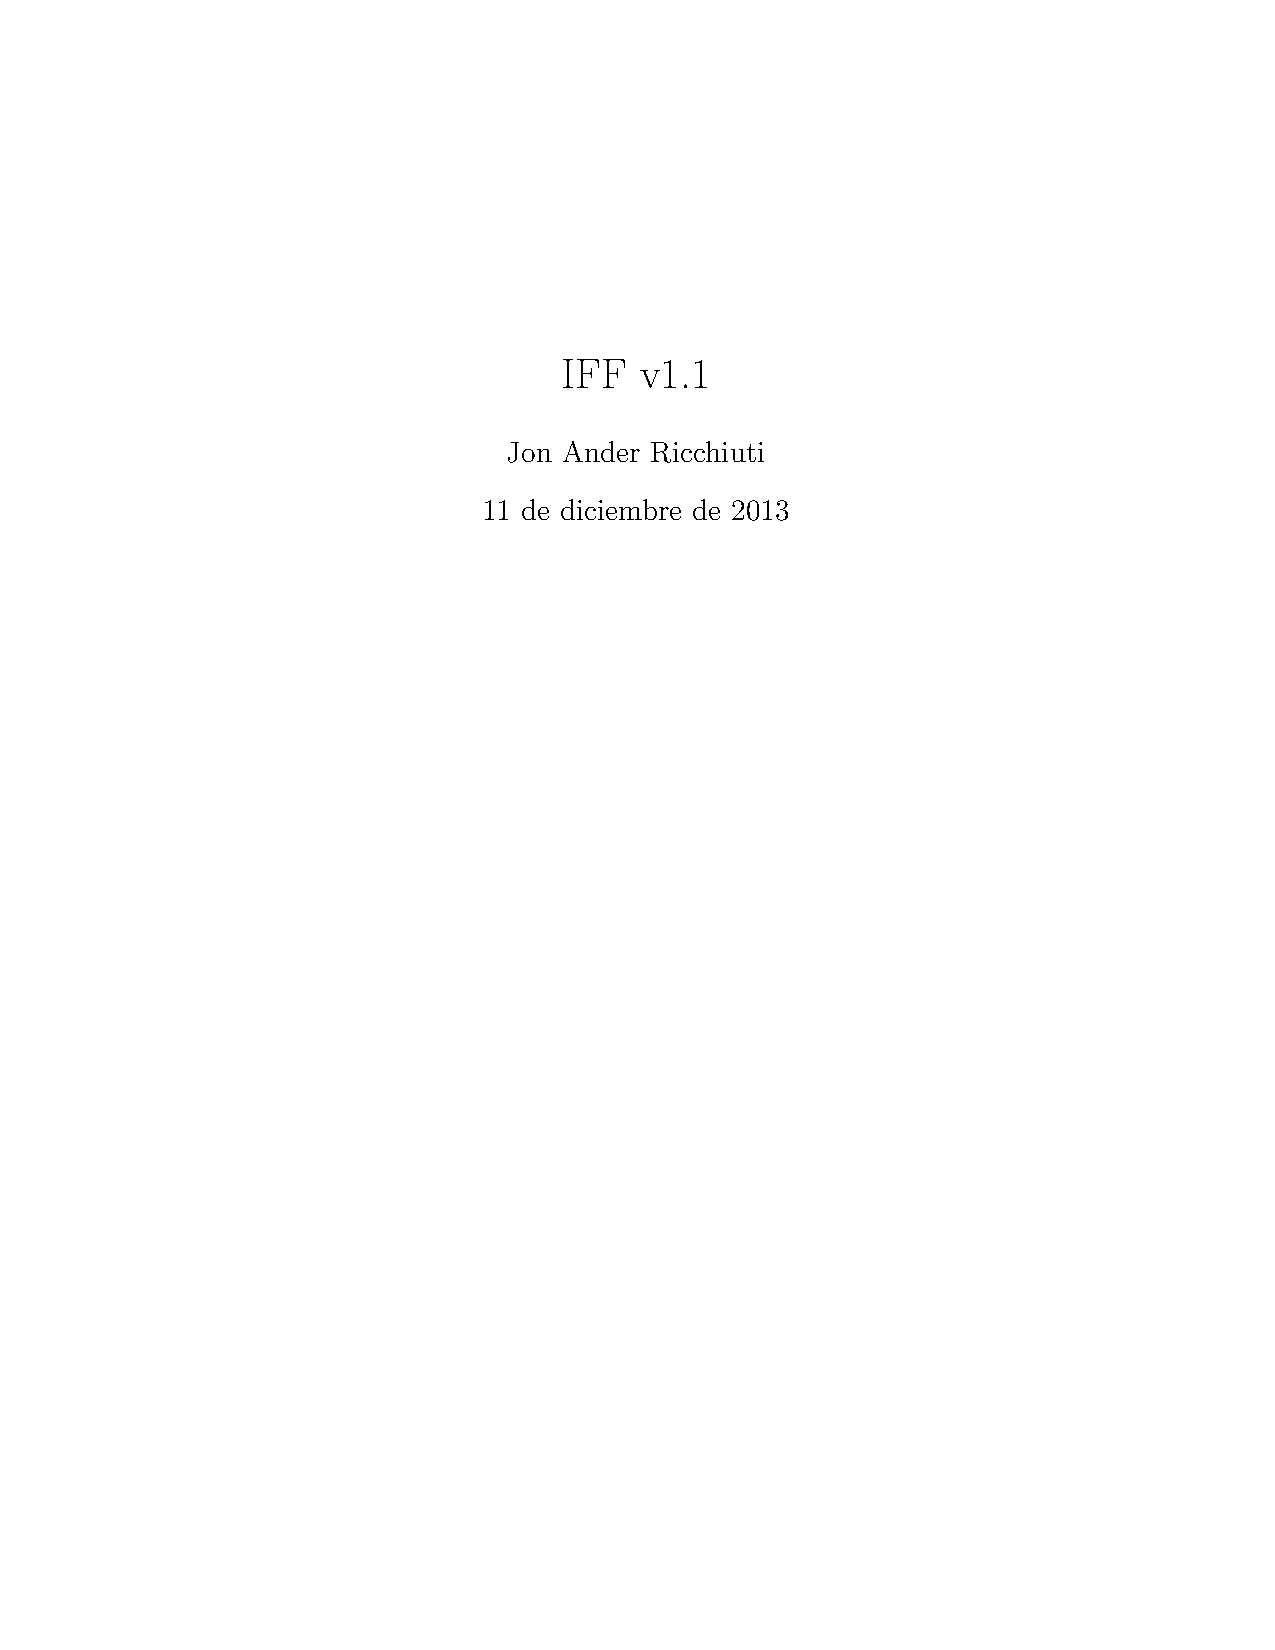
\includepdf[pages=-]{apendices/IFFv1.1/IFF.pdf}
%%\documentclass[12pt,letterpaper]{article}
%\usepackage[utf8]{inputenc}
%\usepackage{amsmath}
%\usepackage{amsfonts}
%\usepackage{amssymb}
%\usepackage[spanish]{babel}
%\usepackage{array}
%\usepackage{longtable}
%\author{Jon Ander Ricchiuti}
%\title{IFF v1.1}
%\begin{document}
%\pagenumbering{arabic}
%\maketitle
%\thispagestyle{empty}
%\newpage
\chapter{Intercambio de Información Financiera (IFF)}

\section*{Introducción}

El protocolo de intercambio de información financiera (IFF), describe la forma correcta de comunicación con un prototipo de sistema bancario creado en Synergy Global Business (SGB). El IFF busca estandarizar el intercambio de información financiera que realizará el prototipo bancario. De esta manera la comunicación es sencilla y a la vez robusta. Para la realización de este protocolo de comunicación se utilizó como base el IFX (Interactive Financial Exchange).
\\
\\ 
La forma de comunicación que el IFF	utiliza es de tipo petición-respuesta (request-response). En cada petición se debe especificar un método. Este método define la naturaleza de la petición.
%\pagenumbering{arabic}
%\newpage

\section{Tipo de datos}

Los tipos de datos que se utilizarán en este estándar son los siguientes:
\begin{itemize}
\item Cadena de caracteres.
\item Enumeración.
\item Tiempo y Hora.
\item Entero.
\item Decimal
\item Booleano.
\end{itemize}

\subsection{Cadena de caracteres}
Las cadenas de caracteres se representan con el nombre de ``Cadena de caracteres'' seguido de la longitud de la misma. Esta longitud es representada entre paréntesis de la siguiente forma.
\begin{itemize}
\item Cadena de caracteres (X-Y), indica que la longitud mínima de la cadena de caracteres es ``X'' y la máxima longitud es ``Y''.
\item Cadena de caracteres (X+), indica que la longitud mínima de la cadena de caracteres es ``X'' pero no tiene longitud máxima para la misma.
\end{itemize}
Si la longitud no es especificada entonces no existe restricción sobre el tamaño de la cadena de caracteres.

\subsection{Enumeración}
Son los valores que puede tomar un campo. Estos pertenecen a un conjunto de cadena de caracteres definidas específicamente para ese campo en particular. Los diferentes tipos de enumeración serán especificados en la siguiente sección.

\subsection{Tiempo y Hora}
Tanto la hora como la fecha son cadenas de caracteres que se representan con un fromato particular. Para la hora el formto es ``\%H:\%M:\%S''. Para la fecha el formato es ``\%Y-\%m-\%d \%H:\%M:\%S''. Donde \%Y representa el año, \%m el mes, \%d el dia, \%H la hora, \%M el minuto, \%S el segundo. Todos los componentes de la hora y fecha se representan con caracteres numéricos.

\subsection{Entero}
Es un número entero y puede representarse de dos formas diferentes. Como un entero de cuatro bytes o como un entero de ocho bytes. Para especificar que es un entero de ocho bytes, debe ser escrito de la siguiente forma: Entero(8).
\\
\\
Si no se especifica que un entero es de ocho bytes entonces se asume que es de cuatro  bytes.

\subsection{Decimal}
Es un número con hasta quince dígitos decimales.

\subsection{Booleano}
Un Booleano representa si una condición se cumple o no. En el caso del IFF un Booleano será representado por medio de un carácter. Es decir, el carácter 'T' será el que representa cuando un estado es cierto y 'F' será el valor de cuando el estado no se cumple.

\section{Tipos de Enumeración}
\subsection{Correspondiente a personVerifyType}
\begin{center}
\begin{tabular}{|>{\centering\arraybackslash}p{0.3\textwidth}|>{\centering\arraybackslash}p{0.3\textwidth}|>{\centering\arraybackslash}p{0.3\textwidth}|}
\hline 
\bfseries {Valor} & \bfseries {Descripción} & \bfseries {Por defecto} \\ 
\hline 
Passport & Pasaporte de crédito & N \\ 
\hline 
CI & Cedula de identidad & N \\
\hline 
\end{tabular} 
\end{center}

\subsection{Correspondiente a nameAddrType}
\begin{center}
\begin{tabular}{|>{\centering\arraybackslash}p{0.3\textwidth}|>{\centering\arraybackslash}p{0.3\textwidth}|>{\centering\arraybackslash}p{0.3\textwidth}|}
\hline 
\bfseries {Valor} & \bfseries {Descripción} & \bfseries {Por defecto} \\ 
\hline 
Customer & Es la dirección del cliente & N \\ 
\hline 
ShipTo & Dirección a la cual algo debería ser enviado por correo & N \\
\hline 
Delivery & Dirección a la cual serán enviadas las facturas en papel & N \\
\hline 
\end{tabular} 
\end{center}

\subsection{Correspondiente a addrType}
\begin{center}
\begin{tabular}{|>{\centering\arraybackslash}p{0.3\textwidth}|>{\centering\arraybackslash}p{0.3\textwidth}|>{\centering\arraybackslash}p{0.3\textwidth}|}
\hline 
\bfseries {Valor} & \bfseries {Descripción} & \bfseries {Por defecto} \\ 
\hline 
Seasonal & Habitación vacacional & N \\ 
\hline 
Primary & Habitación principal & N \\
\hline 
Secondary & Habitación secundaria & N \\
\hline
Business & Dirección de negocio & N \\
\hline 
\end{tabular} 
\end{center}

\subsection{Correspondiente a cardStatusCode}
\begin{center}
\begin{tabular}{|>{\centering\arraybackslash}p{0.3\textwidth}|>{\centering\arraybackslash}p{0.3\textwidth}|>{\centering\arraybackslash}p{0.3\textwidth}|}
\hline 
\bfseries {Valor} & \bfseries {Descripción} & \bfseries {Por defecto} \\ 
\hline 
Active & Activa & N \\ 
\hline 
Expired & Vencida & N \\
\hline 
Blocked & Bloqueada & N \\
\hline
\end{tabular} 
\end{center}

\subsection{Correspondiente a accountStatusCode}
\begin{center}
\begin{tabular}{|>{\centering\arraybackslash}p{0.3\textwidth}|>{\centering\arraybackslash}p{0.3\textwidth}|>{\centering\arraybackslash}p{0.3\textwidth}|}
\hline 
\bfseries {Valor} & \bfseries {Descripción} & \bfseries {Por defecto} \\ 
\hline 
Active & Activa & N \\ 
\hline 
Blocked & Bloqueada & N \\
\hline
\end{tabular} 
\end{center}

\subsection{Correspondiente a cardType}
\begin{center}
\begin{tabular}{|>{\centering\arraybackslash}p{0.3\textwidth}|>{\centering\arraybackslash}p{0.3\textwidth}|>{\centering\arraybackslash}p{0.3\textwidth}|}
\hline 
\bfseries {Valor} & \bfseries {Descripción} & \bfseries {Por defecto} \\ 
\hline 
Credit & Tarjeta de crédito & N \\ 
\hline 
Debit & Tarjeta de débito & N \\
\hline 
\end{tabular} 
\end{center}

\subsection{Correspondiente a brand}
\begin{center}
\begin{tabular}{|>{\centering\arraybackslash}p{0.3\textwidth}|>{\centering\arraybackslash}p{0.3\textwidth}|>{\centering\arraybackslash}p{0.3\textwidth}|}
\hline 
\bfseries {Valor} & \bfseries {Descripción} & \bfseries {Por defecto} \\ 
\hline 
Visa &  & N \\ 
\hline 
MasterCard &  & N \\
\hline 
\end{tabular} 
\end{center}

\subsection{Correspondiente a transType}
\begin{center}
\begin{tabular}{|>{\centering\arraybackslash}p{0.3\textwidth}|>{\centering\arraybackslash}p{0.3\textwidth}|>{\centering\arraybackslash}p{0.3\textwidth}|}
\hline 
\bfseries {Valor} & \bfseries {Descripción} & \bfseries {Por defecto} \\ 
\hline 
Withdrawal & Retiro & N \\ 
\hline 
Deposit & Deposito & N \\
\hline 
Transference & Transferencia & N \\
\hline
\end{tabular} 
\end{center}

\subsection{Correspondiente a acctType}
\begin{center}
\begin{tabular}{|>{\centering\arraybackslash}p{0.3\textwidth}|>{\centering\arraybackslash}p{0.3\textwidth}|>{\centering\arraybackslash}p{0.3\textwidth}|}
\hline 
\bfseries {Valor} & \bfseries {Descripción} & \bfseries {Por defecto} \\ 
\hline 
Saving & Ahorro & N \\ 
\hline 
Current & Corriente & N \\
\hline 
Loan & Préstamo & N \\
\hline
\end{tabular} 
\end{center}

\subsection{Correspondiente a contactInfo}
\begin{center}
\begin{tabular}{|>{\centering\arraybackslash}p{0.3\textwidth}|>{\centering\arraybackslash}p{0.3\textwidth}|>{\centering\arraybackslash}p{0.3\textwidth}|}
\hline 
\bfseries {Valor} & \bfseries {Descripción} & \bfseries {Por defecto} \\ 
\hline 
dayPhone & Teléfono de contacto durante el día & N \\
\hline 
evePhone & Teléfono de contacto durante la tarde & N \\
\hline 
dayFax & Fax de contacto durante el día & N \\
\hline
eveFax & Fax de contacto durante la tarde & N \\
\hline
emailAddr & Dirección de correo electrónica & N \\
\hline
\end{tabular} 
\end{center}
	
\section{Recursos}
El protocolo IFF esta basado en recursos. Los recursos son fuentes de información sobre las cuales se realizan las peticiones. Estos recursos son divididos en dos grandes grupos, los concretos y los abstractos.

\subsection{Recursos concretos}
Los recursos concretos son la representación directa del modelo de datos que expone el core bancario para ofrecer sus servicios. Este tipo de recursos es muy sencillo y son los que permiten realizar las operaciones más básicas. \\

A continuación se presentan los recursos concretos.

\subsubsection{Nombre de usuario ``login''}
Contiene la información que relaciona el nombre de usuario electrónico con su información  en la institución financiera.

\begin{center}
\begin{tabular}{|>{\centering\arraybackslash}p{0.2\textwidth}|>{\centering\arraybackslash}p{0.2\textwidth}|>{\centering\arraybackslash}p{0.2\textwidth}|>{\centering\arraybackslash}p{0.2\textwidth}|}
\hline 
\bfseries {Etiqueta} & \bfseries {Tipo} & \bfseries {Uso} & \bfseries {Descripción} \\ 
\hline 
username & Cadena de caracteres (6-20) & Requerido & ID de ingreso del cliente \\ 
\hline 
password & Cadena de caracteres (6+) & Opcional & Clave de ingreso \\ 
\hline 
custPermId & Cadena de caracteres (32+) & Requerido & ID permanente del cliente. Es asignado por la institución financiera para representar al cliente en el sistema \\ 
\hline 
\end{tabular}
\end{center}

\subsubsection{Cliente ``customer''}
Tiene la información que identifica inequívocamente a un cliente.

\begin{center}
\begin{longtable}{|>{\centering\arraybackslash}p{0.25\textwidth}|>{\centering\arraybackslash}p{0.2\textwidth}|>{\centering\arraybackslash}p{0.15\textwidth}|>{\centering\arraybackslash}p{0.2\textwidth}|}
\hline 
\bfseries {Etiqueta} & \bfseries {Tipo} & \bfseries {Uso} & \bfseries {Descripción} \\ 
\hline 
custPermId & Cadena de caracteres (32+) & Opcional & ID permanente del cliente. Es asignado por la institución financiera para representar al cliente en el sistema \\ 
\hline 
personId & Cadena de caracteres (32+) & Opcional & Relación al objeto ``person'' \\ 
\hline 
custLogin & Cadena de caracteres (6-20) & Opcional & ID permanente del cliente. Es asignado por la institución financiera para representar al cliente en el sistema \\ 
\hline 
personalIdent & Cadena de caracteres (8+) & Requerido & Identificación personal presentada por el cliente \\ 
\hline 
personVerifyType & Enumeración & Requerido & El tipo de documento con el cual se verifica la identidad del cliente \\ 
\hline
dtBCustomer & Fecha & Opcional & Momento en el cual la persona se vuelve cliente de la institución \\ 
\hline
dtLLogin & Fecha & Opcional & Último momento en el cual el cliente utiliza su cuenta \\ 
\hline
group & Cadena de caracteres (32+) & Opcional & Relaciona al cliente con el objeto ``grupo'' \\ 
\hline
\end{longtable}
\end{center}

\subsubsection{Información del banco ``bankInformation''}
Agrupa la información esencial de una agencia bancaria.

\begin{center}
\begin{longtable}{|>{\centering\arraybackslash}p{0.2\textwidth}|>{\centering\arraybackslash}p{0.2\textwidth}|>{\centering\arraybackslash}p{0.2\textwidth}|>{\centering\arraybackslash}p{0.2\textwidth}|}
\hline 
\bfseries {Etiqueta} & \bfseries {Tipo} & \bfseries {Uso} & \bfseries {Descripción} \\ 
\hline 
bankId & Cadena de caracteres (4+) & Opcional & ID que identifica a la agencia bancaria \\ 
\hline 
name & Cadena de caracteres & Opcional & Nombre de la agencia \\ 
\hline 
branchId & Cadena de caracteres & Opcional & ID que identifica a la sucursal \\ 
\hline 
branchName & Cadena de caracteres & Opcional & Nombre de la sucursal \\ 
\hline 
postAddr & Cadena de caracteres & Opcional & Dirección \\ 
\hline
city & Cadena de caracteres & Opcional & Ciudad \\ 
\hline
stateProv & Cadena de caracteres & Opcional & Estado o Provincia \\ 
\hline
postalCode &  Cadena de caracteres (4+) & Opcional & Código postal \\ 
\hline
country & Cadena de caracteres & Opcional & País \\ 
\hline
\end{longtable}
\end{center}

\subsubsection{Dirección ``address''}
Representa la dirección suministrada por el cliente.

\begin{center}
\begin{longtable}{|>{\centering\arraybackslash}p{0.2\textwidth}|>{\centering\arraybackslash}p{0.2\textwidth}|>{\centering\arraybackslash}p{0.2\textwidth}|>{\centering\arraybackslash}p{0.2\textwidth}|}
\hline 
\bfseries {Etiqueta} & \bfseries {Tipo} & \bfseries {Uso} & \bfseries {Descripción} \\ 
\hline 
addressId & Cadena de caracteres & Opcional & ID que identifica a la dirección \\ 
\hline 
custPermId & Cadena de caracteres (32+) & Requerido & ID permanente del cliente. Es asignado por la institución financiera para representar al cliente en el sistema \\
\hline 
nameAddrType & Enumeración & Requerido & Define el uso de la información suministrada \\ 
\hline 
addr & Cadena de caracteres & Opcional & Dirección \\ 
\hline
city & Cadena de caracteres & Opcional & Ciudad \\ 
\hline
stateProv & Cadena de caracteres & Opcional & Estado o Provincia \\ 
\hline
postalCode &  Cadena de caracteres (4+) & Opcional & Código postal \\ 
\hline
country & Cadena de caracteres & Opcional & País \\ 
\hline
addrType & Enumeración & Opcional & Define el tipo de dirección \\ 
\hline
startDt & Hora & Opcional & Hora de inicio \\ 
\hline
endDt & Hora & Opcional & Hora de fin \\ 
\hline
\end{longtable}
\end{center}

\subsubsection{Información de contacto ``contactInfo''}
Información suministrada por el cliente para poder ser contactado en caso de necesitarlo.

\begin{center}
\begin{longtable}{|>{\centering\arraybackslash}p{0.25\textwidth}|>{\centering\arraybackslash}p{0.2\textwidth}|>{\centering\arraybackslash}p{0.15\textwidth}|>{\centering\arraybackslash}p{0.2\textwidth}|}
\hline 
\bfseries {Etiqueta} & \bfseries {Tipo} & \bfseries {Uso} & \bfseries {Descripción} \\ 
\hline 
contactInfoId & Cadena de caracteres (32+) & Opcional & ID que identifica la información de contacto del cliente \\ 
\hline 
custPermId & Cadena de caracteres (32+) & Requerido & ID permanente del cliente. Es asignado por la institución financiera para representar al cliente en el sistema \\
\hline 
custContactPref & Enumeración & Requerido & Representa la manera en la cual el cliente será contactado \\ 
\hline 
prefTimeStart & Hora & Opcional & Hora a partir de la cual puede ser contactado \\ 
\hline
prefTimeEnd & Hora de caracteres & Opcional & Hora a partir de la cual ya no puede ser contactado \\ 
\hline
dayPhone & Cadena de caracteres & Opcional (ver descripción) & Teléfono de contacto durante el día. 
\\ & & & \\
& & & Este campo es requerido si ni ``evePhone'', ``dayFax'', ``eveFax'' o ``emailAddr'' es suministrado \\ 
\hline
evePhone & Cadena de caracteres & Opcional (ver descripción) & Teléfono de contacto durante la tarde. \\ & & & \\
& & & Este campo es requerido si ni ``dayPhone'', ``dayFax'', ``eveFax'' o ``emailAddr'' es suministrado \\ 
\hline
dayFax & Cadena de caracteres & Opcional (ver descripción) & Fax de contacto durante el día. \\ & & & \\
& & & Este campo es requerido si ni ``dayPhone'', ``evePhone'', ``eveFax'' o ``emailAddr'' es suministrado \\ 
\hline
eveFax & Cadena de caracteres & Opcional (ver descripción) & Fax de contacto durante la tarde. \\ & & & \\
& & & Este campo es requerido si ni ``dayPhone'', ``evePhone'', ``dayFax'' o ``emailAddr'' es suministrado \\ 
\hline
emailAddr & Cadena de caracteres & Opcional (ver descripción) & Correo electrónico de contacto. \\ & & & \\
& & & Este campo es requerido si ni ``dayPhone'', ``evePhone'', ``dayFax'' o ``eveFax'' es suministrado \\ 
\hline
\end{longtable}
\end{center}

\subsubsection{Información personal ``personalInfo''}
Contiene la información personal de un cliente.

\begin{center}
\begin{longtable}{|>{\centering\arraybackslash}p{0.2\textwidth}|>{\centering\arraybackslash}p{0.2\textwidth}|>{\centering\arraybackslash}p{0.2\textwidth}|>{\centering\arraybackslash}p{0.2\textwidth}|}
\hline 
\bfseries {Etiqueta} & \bfseries {Tipo} & \bfseries {Uso} & \bfseries {Descripción} \\ 
\hline 
personalInfoId & Cadena de caracteres (32+) & Opcional & ID que identifica a la información personal del cliente \\ 
\hline 
custPermId & Cadena de caracteres (32+) & Requerido & ID permanente del cliente. Es asignado por la institución financiera para representar al cliente en el sistema \\
\hline 
lastName & Cadena de caracteres & Requerido & Apellido del cliente \\ 
\hline 
firstName & Cadena de caracteres & Requerido & Dirección \\ 
\hline
middleName & Cadena de caracteres & Opcional & Ciudad \\ 
\hline
tittlePrefix & Cadena de caracteres & Opcional & Titulo por el cual llamar al cliente. Por ejemplo ``Dr.'' \\ 
\hline
nameSuffix & Cadena de caracteres & Opcional & Sufijo agregado al final del nombre del cliente. Por ejemplo ``Jr.'' \\ 
\hline
\end{longtable}
\end{center}

\subsubsection{Preferencia ``preference''}
Permite al cliente definir cierto comportamiento sobre su cuenta. El cliente puede establecer un monto predeterminado para concepto de retiro sobre una de sus cuentas. También, si se le ha hecho una transferencia al cliente y no se especificó cuenta destino, el dinero será transferido a la cuenta que el cliente haya definido por defecto.

\begin{center}
\begin{longtable}{|>{\centering\arraybackslash}p{0.3\textwidth}|>{\centering\arraybackslash}p{0.15\textwidth}|>{\centering\arraybackslash}p{0.15\textwidth}|>{\centering\arraybackslash}p{0.2\textwidth}|}
\hline 
\bfseries {Etiqueta} & \bfseries {Tipo} & \bfseries {Uso} & \bfseries {Descripción} \\ 
\hline 
preferenceId & Cadena de caracteres (32+) & Opcional & ID que identifica a la información de preferencia del cliente \\ 
\hline 
custPermId & Cadena de caracteres (32+) & Requerido & ID permanente del cliente. Es asignado por la institución financiera para representar al cliente en el sistema \\
\hline 
acctId & Cadena de caracteres (32+) & Opcional & ID de la cuenta a la cual se le aplicaran los consumos por concepto de retiros predefinidos \\ 
\hline 
defaultTranfAccount & Cadena de caracteres (32+) & Opcional & ID de la cuenta a la cual se le aplicaran las transferencias sin cuenta de destino especificada \\ 
\hline
withdrawalAmt & Cadena de caracteres (32+) & Opcional (ver descripción) & Monto de retiro por defecto. 
\\ & & & \\
& & & Este campo es requerido si ``acctId'' es especificado \\
\hline
\end{longtable}
\end{center}

\subsubsection{Transferencias a terceros ``registeredRecipient''}
Contiene los datos de alguna cuenta o tarjeta de otro banco junto con la identificación de sus acreedores.

\begin{center}
\begin{longtable}{|>{\centering\arraybackslash}p{0.25\textwidth}|>{\centering\arraybackslash}p{0.2\textwidth}|>{\centering\arraybackslash}p{0.15\textwidth}|>{\centering\arraybackslash}p{0.2\textwidth}|}
\hline 
\bfseries {Etiqueta} & \bfseries {Tipo} & \bfseries {Uso} & \bfseries {Descripción} \\ 
\hline 
recipientId & Cadena de caracteres (32+) & Opcional & ID que identifica la información acerca de un cliente en otra institución financiera \\ 
\hline 
custPermId & Cadena de caracteres (32+) & Requerido & ID permanente del cliente. Es asignado por la institución financiera para representar al cliente en el sistema \\
\hline 
personId & Cadena de caracteres (32+) & Opcional & ID que identifica al objeto ``person'' \\ 
\hline 
acctNum & Cadena de caracteres & Opcional (ver descripción) & representa el número de cuenta en alguna otra institución financiera. 
\\ & & & \\
& & & Este campo es requerido si ``cardSeqNum'' no es especificado \\ 
\hline
cardSeqNum & Cadena de caracteres & Opcional (ver descripción) & representa el número de tarjeta de alguna otra institución financiera. 
\\ & & & \\
& & & Este campo es requerido si ``acctNum'' no es especificado \\ 
\hline
name & Cadena de caracteres & Requerido & Nombre del beneficiario \\ 
\hline
desc & Cadena de caracteres & Requerido & Descripción \\ 
\hline
maxAmtLimit & Cadena de caracteres & Opcional & Máximo monto permitido para realizar la transferencia \\ 
\hline
personalIdent & Cadena de caracteres (8+) & Requerido & Identificación personal presentada por el cliente \\ 
\hline
personVerifyType & Enumeración & Requerido & El tipo de documento con el cual se verifica la identidad del cliente \\ 
\hline
\end{longtable}
\end{center}

\subsubsection{Persona ``person''}
Contiene los datos que identifican a los clientes como personas. También reúne los
datos de los clientes que tienen cuentas en otros bancos, estos datos provienen de
``registeredRecipient''.

\begin{center}
\begin{longtable}{|>{\centering\arraybackslash}p{0.3\textwidth}|>{\centering\arraybackslash}p{0.15\textwidth}|>{\centering\arraybackslash}p{0.15\textwidth}|>{\centering\arraybackslash}p{0.2\textwidth}|}
\hline 
\bfseries {Etiqueta} & \bfseries {Tipo} & \bfseries {Uso} & \bfseries {Descripción} \\ 
\hline 
personId & Cadena de caracteres (32+) & Opcional & ID que identifica a la información de una persona \\ 
\hline 
name & Cadena de caracteres & Requerido & Nombre \\
\hline 
\end{longtable}
\end{center}

\subsubsection{Conocido ``known''}
Contiene la información de las personas conocidas. De esta forma se puede pueden
realizar transferencias a personas en lugar de a cuentas.

\begin{center}
\begin{longtable}{|>{\centering\arraybackslash}p{0.3\textwidth}|>{\centering\arraybackslash}p{0.15\textwidth}|>{\centering\arraybackslash}p{0.15\textwidth}|>{\centering\arraybackslash}p{0.2\textwidth}|}
\hline 
\bfseries {Etiqueta} & \bfseries {Tipo} & \bfseries {Uso} & \bfseries {Descripción} \\ 
\hline 
knownId & Cadena de caracteres (32+) & Opcional & ID que identifica a la información acerca de un conocido	 \\ 
\hline 
personId & Cadena de caracteres (32+) & Requerido & ID que identifica la información acerca de una persona.
\\ & & & \\
& & & En este caso representa a un conocido \\
\hline 
custPermId & Cadena de caracteres (32) & Requerido & ID permanente del cliente. Es asignado por la institución financiera para representar al cliente en el sistema.
\\ & & & \\
& & & En este caso representa al conocedor \\
\hline 
relationship & Cadena de caracteres & Requerido & Describe el tipo de relación entre el conocedor y el conocido. \\ 
\hline 
status & Booleano & Opcional & Representa si se ha validado que estas dos personas se conocen \\ 
\hline 
\end{longtable}
\end{center}

\subsubsection{Miembro de un grupo ``groupMember''}
Un cliente tiene la capacidad de crear grupo de personas conocidas. De esta forma puede establecer en que cuenta serán ubicados los fondos recibidos por parte de algún miembro del grupo. Un miembro del grupo es aquel cliente que pertenezca a un grupo.

\begin{center}
\begin{longtable}{|>{\centering\arraybackslash}p{0.25\textwidth}|>{\centering\arraybackslash}p{0.2\textwidth}|>{\centering\arraybackslash}p{0.15\textwidth}|>{\centering\arraybackslash}p{0.2\textwidth}|}
\hline 
\bfseries {Etiqueta} & \bfseries {Tipo} & \bfseries {Uso} & \bfseries {Descripción} \\ 
\hline 
groupMemberId & Cadena de caracteres (32+) & Opcional & ID que identifica al objeto ``groupMember'' \\ 
\hline 
custPermId & Cadena de caracteres (32+) & Requerido & ID permanente del cliente. Es asignado por la institución financiera para representar al cliente en el sistema \\
\hline 
member & Cadena de caracteres (32+) & Requerido & Representa al cliente miembro del grupo \\
\hline 
groupId & Cadena de caracteres (32+) & Requerido & Identifica al grupo al cual pertenece un miembro de grupo\\
\hline 
\end{longtable}
\end{center}

\subsubsection{Grupo ``group''}
Es una unidad en la cual un cliente puede agrupar a otros clientes del banco y
predefinir una cuenta en la cual los miembros al grupo transferirán.

\begin{center}
\begin{longtable}{|>{\centering\arraybackslash}p{0.2\textwidth}|>{\centering\arraybackslash}p{0.2\textwidth}|>{\centering\arraybackslash}p{0.2\textwidth}|>{\centering\arraybackslash}p{0.2\textwidth}|}
\hline 
\bfseries {Etiqueta} & \bfseries {Tipo} & \bfseries {Uso} & \bfseries {Descripción} \\ 
\hline 
groupId & Cadena de caracteres (32+) & Opcional & ID que identifica al objeto ``group'' \\ 
\hline
acctId & Cadena de caracteres (32+) & Opcional & ID de la cuenta a la cual se le aplicaran los consumos por concepto de retiros predefinidos \\ 
\hline 
name & Cadena de caracteres & Requerido & Nombre del grupo \\
\hline 
descripción & Cadena de caracteres & Opcional & Descripción del grupo \\
\hline 
\end{longtable}
\end{center}

\subsubsection{Estado de la cuenta ``accountStatus''}
Tiene la información del estado en el cual se encuentra la cuenta.

\begin{center}
\begin{longtable}{|>{\centering\arraybackslash}p{0.25\textwidth}|>{\centering\arraybackslash}p{0.2\textwidth}|>{\centering\arraybackslash}p{0.15\textwidth}|>{\centering\arraybackslash}p{0.2\textwidth}|}
\hline 
\bfseries {Etiqueta} & \bfseries {Tipo} & \bfseries {Uso} & \bfseries {Descripción} \\ 
\hline 
accountStatusId & Cadena de caracteres (32+) & Opcional & ID que identifica al objeto ``accountStatus'' \\ 
\hline
acctId & Cadena de caracteres (32+) & Opcional & ID de la cuenta a la cual se le aplicaran los consumos por concepto de retiros predefinidos \\ 
\hline 
accountStatusCode & Enumeración & Requerido & Representa el estado de la cuenta \\
\hline 
effDt & Fecha & Opcional & Fecha en la cual se hizo efectivo dicho estado \\
\hline 
statusModBy & Cadena de caracteres & Opcional & Tiene la información acerca de quien modificó el estado \\
\hline 
statusDesc & Cadena de caracteres & Opcional & Descripción sobre el estado \\
\hline 
\end{longtable}
\end{center}

\subsubsection{Estado de la tarjeta ``cardStatus''}
Contiene la información del estado en el cual se encuentra la tarjeta.

\begin{center}
\begin{longtable}{|>{\centering\arraybackslash}p{0.25\textwidth}|>{\centering\arraybackslash}p{0.2\textwidth}|>{\centering\arraybackslash}p{0.15\textwidth}|>{\centering\arraybackslash}p{0.2\textwidth}|}
\hline 
\bfseries {Etiqueta} & \bfseries {Tipo} & \bfseries {Uso} & \bfseries {Descripción} \\ 
\hline 
card	StatusId & Cadena de caracteres (32+) & Opcional & ID que identifica al objeto ``cardStatus'' \\ 
\hline
cardEmBossNum & Cadena de caracteres (32+) & Requerido & Número de la tarjeta a la cual pertenece el estado \\ 
\hline 
cardStatusCode & Enumeración & Requerido & Representa el estado de la tarjeta \\
\hline 
effDt & Fecha & Opcional & Fecha en la cual se hizo efectivo dicho estado \\
\hline 
statusModBy & Cadena de caracteres & Opcional & Tiene la información acerca de quien modificó el estado \\
\hline 
statusDesc & Cadena de caracteres & Opcional & Descripción sobre el estado \\
\hline 
\end{longtable}
\end{center}

\subsubsection{Tarjeta ``card''}
Contiene la información de la tarjeta.

\begin{center}
\begin{longtable}{|>{\centering\arraybackslash}p{0.25\textwidth}|>{\centering\arraybackslash}p{0.2\textwidth}|>{\centering\arraybackslash}p{0.15\textwidth}|>{\centering\arraybackslash}p{0.2\textwidth}|}
\hline 
\bfseries {Etiqueta} & \bfseries {Tipo} & \bfseries {Uso} & \bfseries {Descripción} \\ 
\hline 
cardEmBossNum & Cadena de caracteres (32+) & Requerido & Número de la tarjeta \\ 
\hline
acctId & Cadena de caracteres (32+) & Requerido & ID de la cuenta a la cual se le aplicaran los consumos por concepto de retiros predefinidos \\ 
\hline
cardType & Enumeración & Opcional & Tipo de tarjeta \\
\hline 
brand & Enumeración & Opcional & Consorcio al que pertenece la tarjeta \\
\hline 
issuerName & Cadena de caracteres & Opcional & Nombre del tarjetahabiente \\
\hline 
issDt & Fecha & Opcional & Fecha en la cual se emite la tarjeta \\
\hline 
expDt & Fecha & Opcional & Fecha en la cual expira la tarjeta \\
\hline 
\end{longtable}
\end{center}

\subsubsection{Balance ``balance''}
Contiene la información del dinero existente en una cuenta y las transacciones que
la han afectado.

\begin{center}
\begin{longtable}{|>{\centering\arraybackslash}p{0.2\textwidth}|>{\centering\arraybackslash}p{0.2\textwidth}|>{\centering\arraybackslash}p{0.2\textwidth}|>{\centering\arraybackslash}p{0.2\textwidth}|}
\hline 
\bfseries {Etiqueta} & \bfseries {Tipo} & \bfseries {Uso} & \bfseries {Descripción} \\ 
\hline 
acctId & Cadena de caracteres (32+) & Requerido & ID de la cuenta a la cual pertenece el balance \\ 
\hline
transId & Entero (8) & Opcional & ID de la transacción que afectó el balance \\
\hline 
curAmt & Decimal & Requerido & Cantidad de dinero en la cuenta para la fecha \\
\hline 
effDt & Fecha & requerido & Fecha en la cual se afectó el balance \\
\hline 
descr & Cadena de caracteres & Opcional & Descripción \\
\hline 
\end{longtable}
\end{center}

\subsubsection{Transacción ``transaction''}
Cualquier movimiento que afecte algún balance.

\begin{center}
\begin{longtable}{|>{\centering\arraybackslash}p{0.2\textwidth}|>{\centering\arraybackslash}p{0.2\textwidth}|>{\centering\arraybackslash}p{0.2\textwidth}|>{\centering\arraybackslash}p{0.2\textwidth}|}
\hline 
\bfseries {Etiqueta} & \bfseries {Tipo} & \bfseries {Uso} & \bfseries {Descripción} \\ 
\hline
transId & Entero (8) & Opcional & ID de la transacción \\
\hline 
acctId & Cadena de caracteres (32+) & Requerido & ID de la cuenta que realizó la transacción \\ 
\hline 
acctOutFlow & Cadena de caracteres (32+) & Opcional (ver descripción) & ID de la cuenta a la cual se le debitará el dinero.
\\ & & & \\
& & & Este campo es requerido en caso de que la transacción debite de alguna forma dinero de la cuenta \\
\hline 
acctInFlow & Cadena de caracteres (32+) & Opcional (ver descripción) & ID de la cuenta que recibirá el dinero.
\\ & & & \\
& & & Este campo es requerido en caso de que la transacción abone de alguna forma dinero a la cuenta \\
\hline
thirdParty & Cadena de caracteres & Opcional (ver descripción) & ID de la cuenta o tarjeta de un beneficiario en otro banco.
\\ & & & \\
& & & Este campo es requerido en caso de existir un tercero involucrado \\
\hline
amt & Decimal & Requerido & Cantidad de dinero que moverá la transacción \\
\hline 
dueDt & Fecha & Requerido & Fecha en la cual se desea la transacción sea efectuada \\
\hline 
curDt & Fecha & Requerido & Fecha en la cual se realizó la transacción \\
\hline 
transType & Enumeración & Opcional & Tipo de transacción realizada \\
\hline 
\end{longtable}
\end{center}

\subsubsection{Transacción ``transaction''}
Cualquier movimiento que afecte algún balance.

\begin{center}
\begin{longtable}{|>{\centering\arraybackslash}p{0.2\textwidth}|>{\centering\arraybackslash}p{0.2\textwidth}|>{\centering\arraybackslash}p{0.2\textwidth}|>{\centering\arraybackslash}p{0.2\textwidth}|}
\hline 
\bfseries {Etiqueta} & \bfseries {Tipo} & \bfseries {Uso} & \bfseries {Descripción} \\ 
\hline
acctId & Cadena de caracteres (32+) & Requerido & ID de la cuenta que realizó la transacción \\ 
\hline 
bankId & Cadena de caracteres & Requerido & ID que identifica a la agencia bancaria \\
\hline 
custPermId & Cadena de caracteres (32+) & Requerido & ID permanente del cliente. Es asignado por la institución financiera para representar al cliente en el sistema 
\\ & & & \\
& & & Este campo es requerido si la cuenta no es compartida \\
\hline
acctType & Enumeración & Requerido & Define de qué tipo es la cuenta \\
\hline
freeForAll & Booleano & Opcional (ver descripción) & En caso de que la cuenta sea compartida, define si cualquiera puede efectuar operaciones o se necesita la aprobación de todos los participantes.
\\ & & & \\
& & & Es requerido si el campo ``custPermId'' no está definido \\
\hline 
members & Entero & Opcional (ver descripción) & Define cuantos clientes comparten la cuenta
\\ & & & \\
& & & El campo es requerido si ``freeForAll'' está definido \\
\hline 
\end{longtable}
\end{center}

\subsection{Recursos abstractos}
A diferencia de los recursos concretos, los recursos abstractos no representan objetos en la base de datos. Estos recursos ofrecen una información más general y son producto de una recopilación de información sobre varios objetos en la base de datos. También se pueden utilizar estos recursos para ofrecer una forma más sencilla de actualizar alguna información en el sistema. Por ejemplo, si se desea registrar un nuevo cliente, se tendrían que mandar varias peticiones para crear los recursos necesarios para que el cliente sea registrado. Para evitar mandar varias peticiones se podría ofrecer un recurso que recopile toda la información necesaria y este se encargue de crear los recursos concretos necesarios para que el nuevo cliente pueda ser registrado.
%\end{document}
\chapter{Capturas de pantalla de la aplicación móvil} \label{chap: Screenshots mobile}

\begin{figure}[ht]
\centering
\begin{minipage}{.5\textwidth}
  \centering
  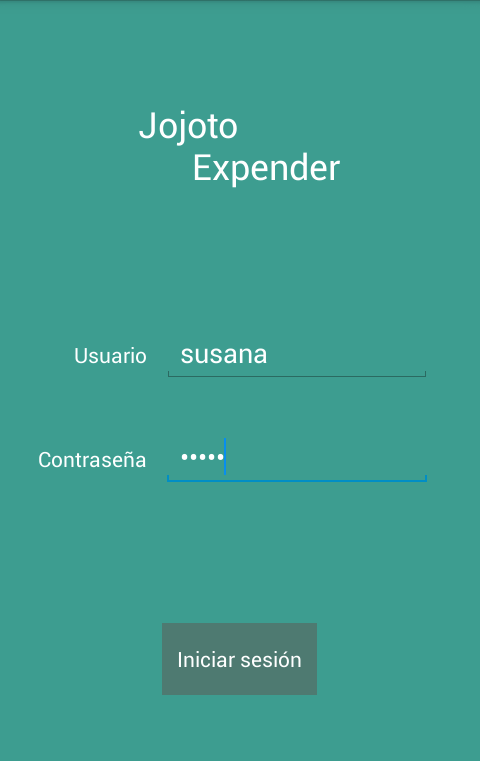
\includegraphics[scale=0.30,type=png,ext=.png,read=.png]{imagenes/Screenshots/login_mobile}
  \captionsetup{justification=centering}
  \captionof{figure}{Interfaz para iniciar sesión}
  \label{fig:interfazLoginMobile}
\end{minipage}%
\begin{minipage}{.5\textwidth}  
\centering
  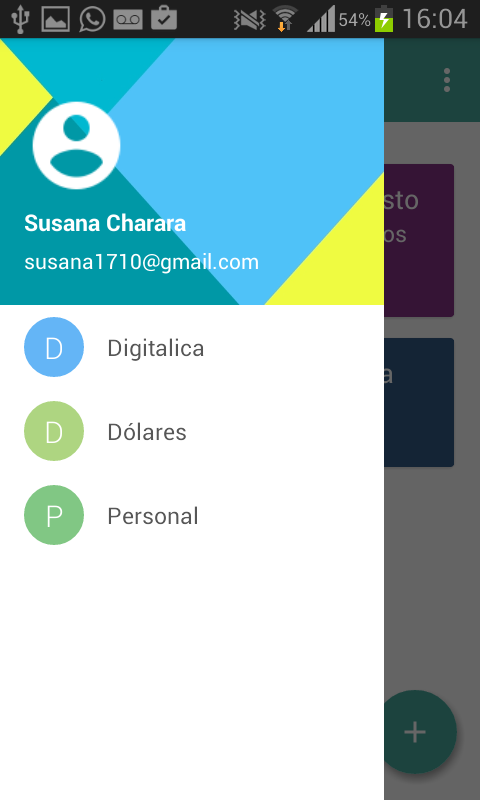
\includegraphics[scale=0.30,type=png,ext=.png,read=.png]{imagenes/Screenshots/sidebar}
  \captionsetup{justification=centering}
  \captionof{figure}{Interfaz para cambiar de cuenta}
  \label{fig:interfazCambiarCuenta}\end{minipage}
\end{figure}

\begin{figure}[ht]
\centering
\begin{minipage}{.5\textwidth}
  \centering
  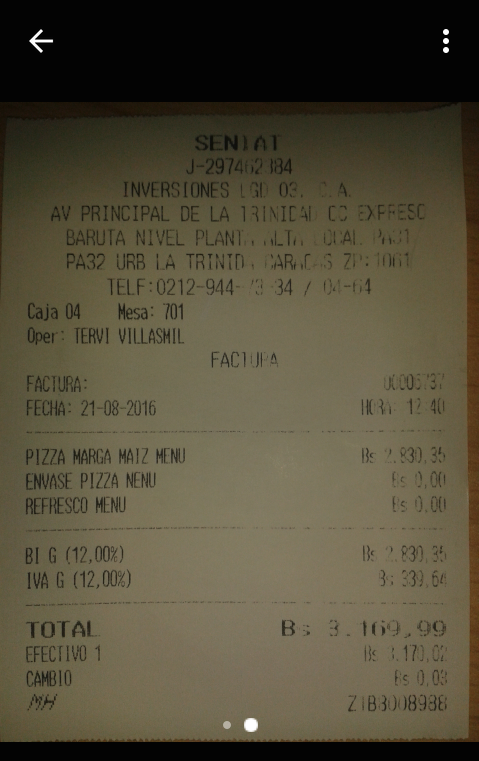
\includegraphics[scale=0.30,type=png,ext=.png,read=.png]{imagenes/Screenshots/photo_view1}
  \captionsetup{justification=centering}
  \captionof{figure}{Interfaz para ver fotos en pantalla completa}
  \label{fig:interfazVerFoto}
\end{minipage}%
\begin{minipage}{.5\textwidth}
\centering
  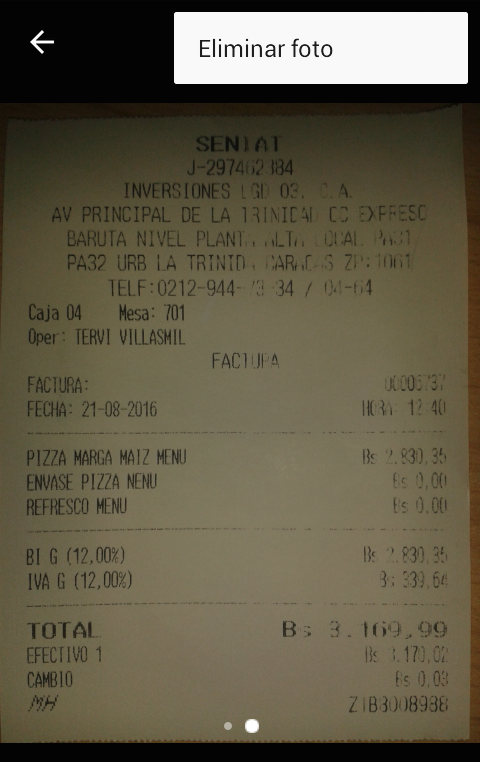
\includegraphics[scale=0.30,type=png,ext=.png,read=.png]{imagenes/Screenshots/photo_view2}
  \captionsetup{justification=centering}
  \captionof{figure}{Interfaz para eliminar\\ fotos}
  \label{fig:interfazEliminarFoto}
\end{minipage}
\end{figure}

\begin{figure}[ht]
\centering
\begin{minipage}{.5\textwidth}
  \centering
  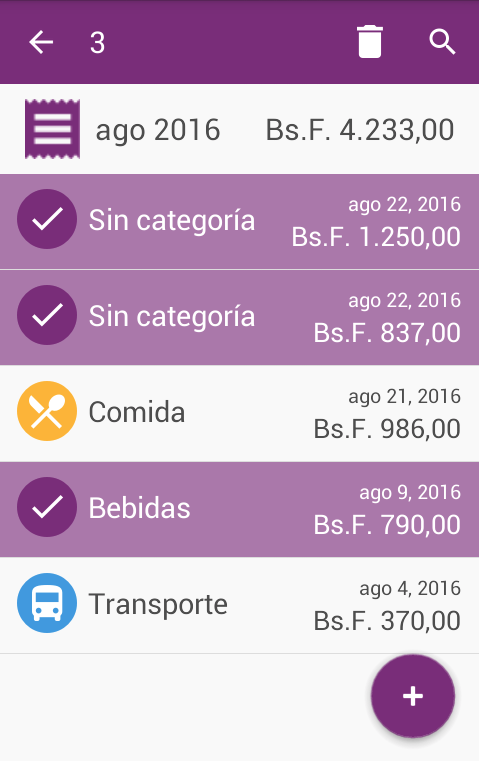
\includegraphics[scale=0.30,type=png,ext=.png,read=.png]{imagenes/Screenshots/select_expenses}
  \captionsetup{justification=centering}
  \captionof{figure}{Interfaz para eliminar gastos}
  \label{fig:interfazEliminarGastos}
\end{minipage}%
\begin{minipage}{.5\textwidth}
\centering
  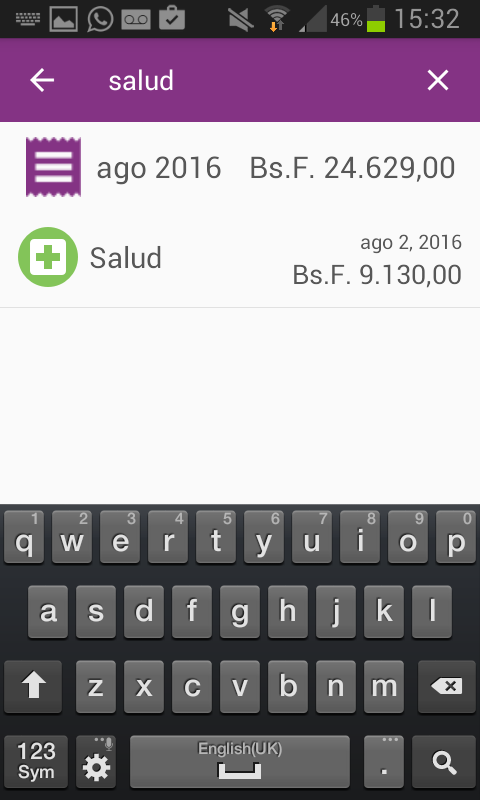
\includegraphics[scale=0.30,type=png,ext=.png,read=.png]{imagenes/Screenshots/filter}
  \captionsetup{justification=centering}
  \captionof{figure}{Interfaz para filtrar gastos}
  \label{fig:interfazFiltrarGastos}
\end{minipage}
\end{figure}

\begin{figure}[ht]
\centering
\begin{minipage}{.5\textwidth}
  \centering
  
\includegraphics[scale=0.30,type=png,ext=.png,read=.png]{imagenes/Screenshots/create_account1}
  \captionsetup{justification=centering}
  \captionof{figure}{Interfaz para crear una cuenta}
  \label{fig:interfazCrearCuenta}
\end{minipage}%
\begin{minipage}{.5\textwidth}
\centering
  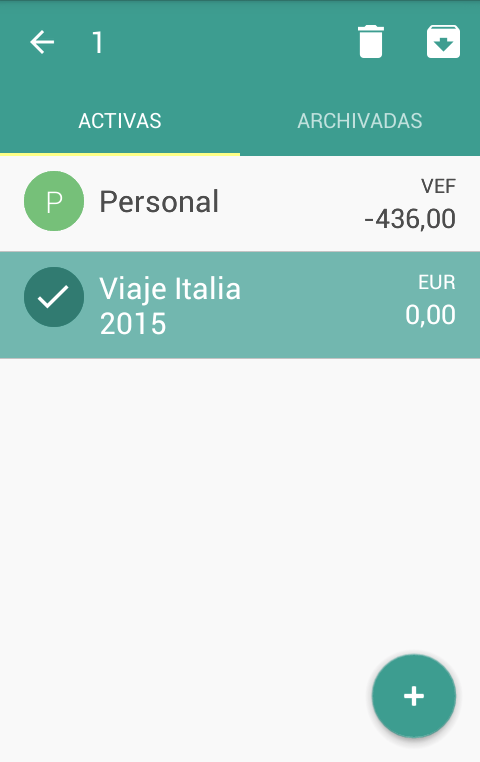
\includegraphics[scale=0.30,type=png,ext=.png,read=.png]{imagenes/Screenshots/select_accounts}
  \captionsetup{justification=centering}
  \captionof{figure}{Interfaz para eliminar cuentas}
  \label{fig:interfazEliminarCuentas}
\end{minipage}
\end{figure}

\begin{figure}[ht]
\centering
\begin{minipage}{.5\textwidth}
  \centering
  
\includegraphics[scale=0.30,type=png,ext=.png,read=.png]{imagenes/Screenshots/create_category1}
  \captionsetup{justification=centering}
  \captionof{figure}{Interfaz para crear una\\ categoría}
  \label{fig:interfazCrearCategoria}
\end{minipage}%
\begin{minipage}{.5\textwidth}
\centering
  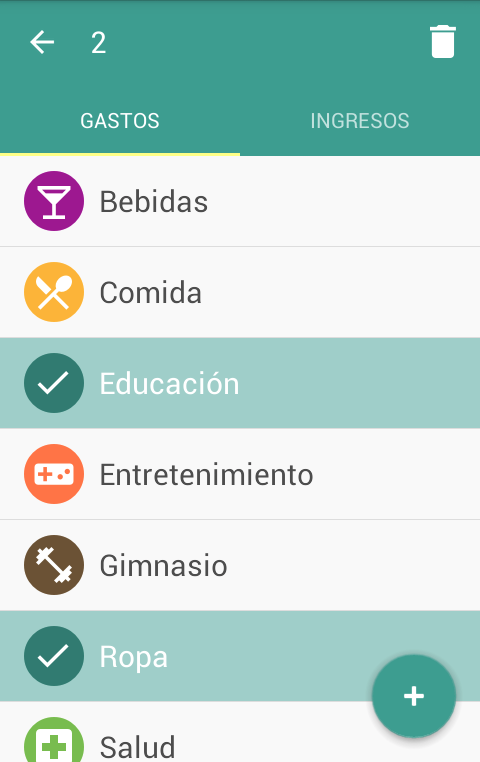
\includegraphics[scale=0.30,type=png,ext=.png,read=.png]{imagenes/Screenshots/select_categories}
  \captionsetup{justification=centering}
  \captionof{figure}{Interfaz para eliminar\\ categorías}
  \label{fig:interfazEliminarCategorias}
\end{minipage}
\end{figure}

\begin{figure}[ht]
\centering
\begin{minipage}{.5\textwidth}
\centering
  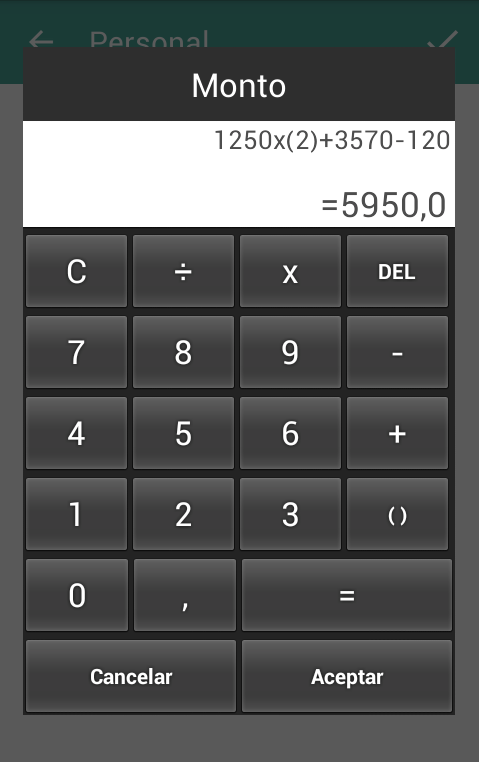
\includegraphics[scale=0.30,type=png,ext=.png,read=.png]{imagenes/Screenshots/calculator}
  \captionsetup{justification=centering}
  \captionof{figure}{Interfaz de la\\ calculadora}
  \label{fig:interfazCalculadora}

\end{minipage}%
\begin{minipage}{.5\textwidth}
\centering
  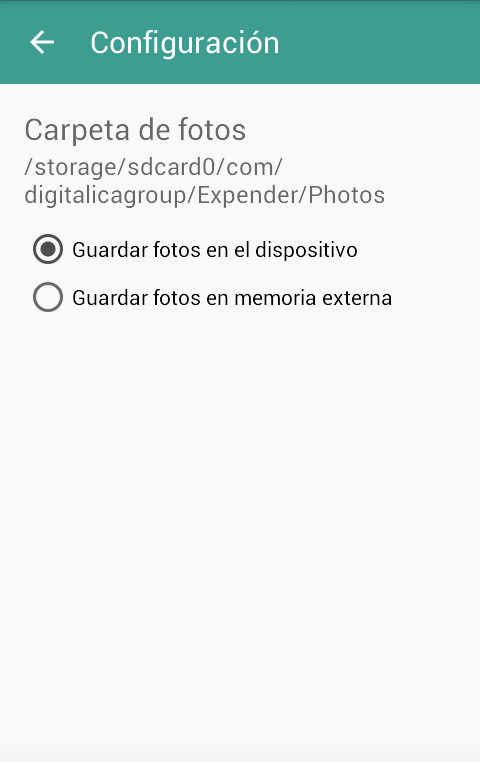
\includegraphics[scale=0.30,type=png,ext=.png,read=.png]{imagenes/Screenshots/configuration}
  \captionsetup{justification=centering}
  \captionof{figure}{Interfaz para cambiar la ubicación de las fotos}
  \label{fig:interfazConfiguracion}
\end{minipage}
\end{figure}
\chapter{Capturas de pantalla de la aplicación web} \label{chap: Screenshots web}

\begin{figure}[ht]
  \centering
  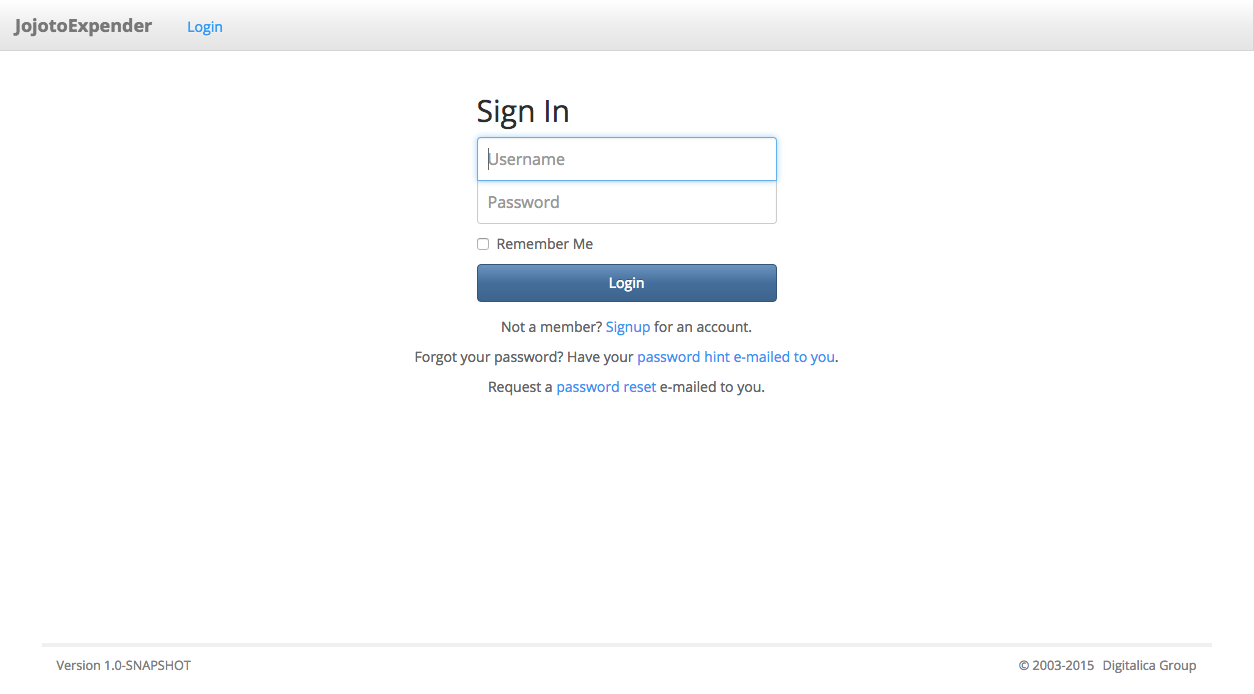
\includegraphics[scale=0.45,type=png,ext=.png,read=.png]{imagenes/login_web}
  \captionsetup{justification=centering}
  \caption{Interfaz para iniciar sesión en la aplicación web}
  \label{fig:interfazLoginWeb}
\end{figure}

\begin{figure}[ht]
  \centering
  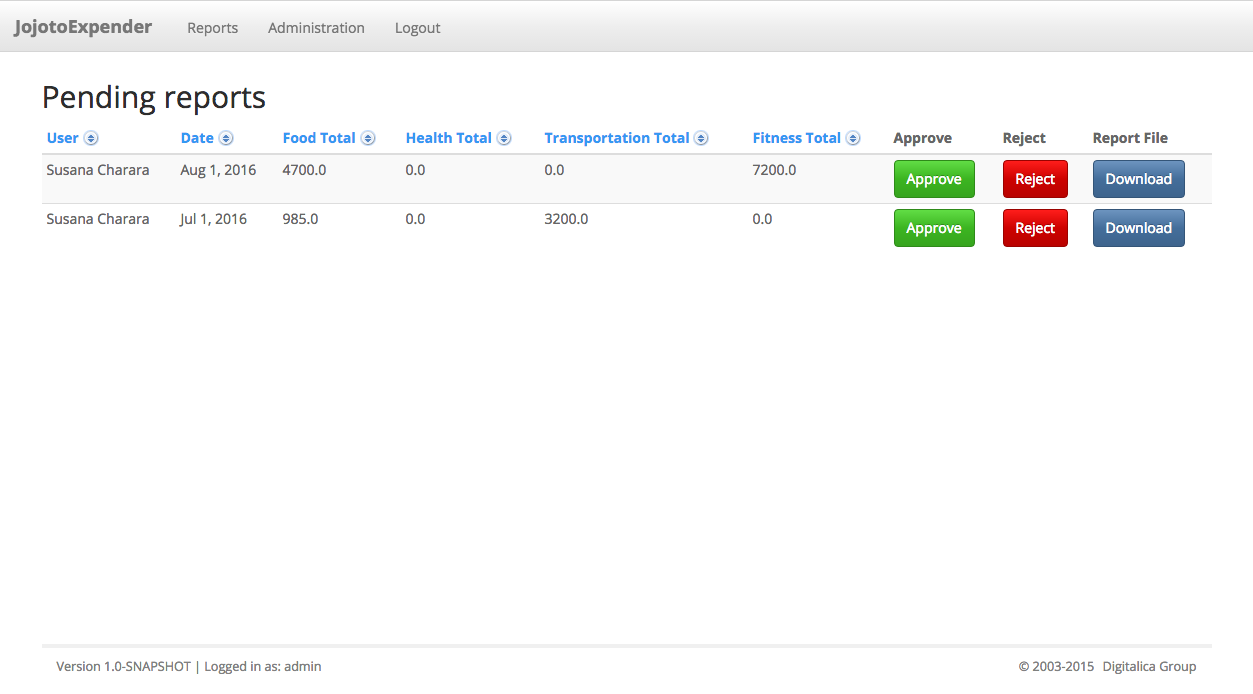
\includegraphics[scale=0.35,type=png,ext=.png,read=.png]{imagenes/pending_reports}
  \captionsetup{justification=centering}
  \caption{Interfaz para listar reportes pendientes de revisión}
  \label{fig:interfazListarReportesPendientesApendice}
\end{figure}

\begin{figure}[h]
  \centering
  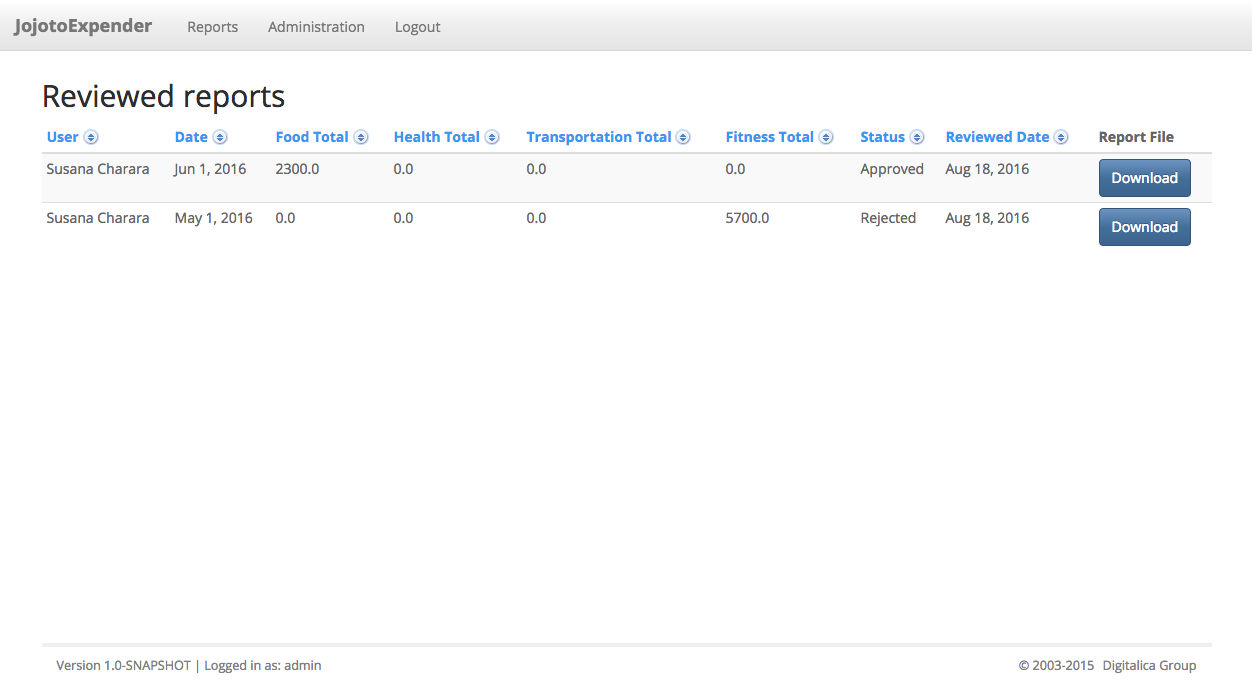
\includegraphics[scale=0.35,type=png,ext=.png,read=.png]{imagenes/reviewed_reports}
  \captionsetup{justification=centering}
  \caption{Interfaz para listar reportes aprobados/rechazados}
  \label{fig:interfazListarReportesRevisadosApendice}
\end{figure}
\chapter{Documento de Historias de Usuario (\textit{Product Backlog})}\label{chap:Product Backlog}

\begin{itemize}
	\item Como USUARIO, quiero ver el Dashboard. %As a USER I want to see the Dashboard.
	\item Como USUARIO, quiero crear un gasto. %As a USER I want to create an Expense.
	
	\item Como USUARIO, quiero crear un ingreso. %As a USER I want to create an Income.
	\item Como USUARIO, quiero tomar fotos de un ingreso o gasto. %As a USER I want to take photo for an Income or Expense.
	\item Como USUARIO, quiero listar mis categorías. %As a USER I want to list my Categories.
	\item Como USUARIO, quiero seleccionar una categoría al crear/editar un ingreso/gasto. %As a USER I want to select a Category when creating/editing an Income/Expenses.
	\item Como USUARIO, quiero ver la lista de ingresos/gastos del mes actual. %As a USER I want to see the list of entries of my expenses/incomes of the current month.
	\item Como USUARIO, quiero ver los detalles de un ingreso/gasto en específico. %As a USER I want to see the details of a specific entry (Expense/Income).
	\item Como USUARIO, quiero editar un ingreso/gasto. %As a USER I want to edit a entry (Expense/Income).
	\item Como USUARIO, quiero eliminar ingresos/gastos. %As a USER I want to delete entries (Expense/Income).
	\item Como USUARIO, quiero tener una calculadora integrada. %As a USER I want to have a built-in calculator.

	\item Como USUARIO, quiero ver mi lista de cuentas. %As a USER I want to see my Account's list.
	\item Como USUARIO, quiero crear una nueva cuenta. %As a USER I want to create a new Account.
	\item Como USUARIO, quiero navegar entre cuentas. %As a USER I want to navigate between Accounts.
	\item Como USUARIO, quiero editar mis cuentas. %As a USER I want to edit my Accounts.
	\item Como USUARIO, quiero eliminar cuentas. %As a USER I want to delete Accounts.
	\item Como USUARIO, quiero archivar una cuenta. %As a USER I want to archive an Account.
	\item Como USUARIO, quiero desarchivar una cuenta. %As a USER I want to unarchive an Account.
	\item Como USUARIO, quiero ver la lista de ingresos/gastos de una cuenta. %As a USER I want to see the entry list of an Account (Account balance).

	\item Como USUARIO, quiero ver las fotos de un ingreso/gasto. %As a USER I want to view the photos of an Entry.
	\item Como USUARIO, quiero eliminar una foto. %As a USER I want to delete a photo.
	\item Como USUARIO, quiero crear una nueva categoría. %As a USER I want to create a new Category.
	\item Como USUARIO, quiero eliminar una categoría. %As a USER I want to delete a Category.
	\item Como USUARIO, quiero editar una categoría. %As a USER I want to edit a Category.
	\item Como USUARIO, quiero cambiar la carpeta de mis fotos. %As a USER I want to set my photo's folder.
	
	\item Como USUARIO, quiero ver mi reporte de balance general. %As a USER I want to see my balance report.
	\item Como USUARIO, quiero ver mi reporte por categoría.%As a USER I want to see a report per Category.
	\item Como USUARIO, quiero compartir mi reporte como un archivo PDF. %As a USER I want to share a report as PDF.
	
	\item Como USUARIO, quiero iniciar sesión con mis credenciales. %As a USER I want to login with my credentials.
	\item Como USUARIO, quiero recibir reportes de gastos de un cliente.%As a USER I want to receive Expense Reports from a client (mobile app).
	\item Como USUARIO, quiero ver la lista de reportes pendientes. %As a USER I want to view the list of pending Reports.
	\item Como USUARIO, quiero aprobar un reporte de gastos.%As a USER I want to approve an expense report.
	\item Como USUARIO, quiero rechazar un reporte de gastos. %As a USER I want to reject a expense report.
	\item Como USUARIO, quiero ver una lista de todos los reportes aprobados y rechazados. %As a USER I want to see a list of all approved and rejected Reports.
	\item Como USUARIO, quiero descargar los detalles de un reporte de gastos en un archivo PDF. %As a USER I want to download the details of an expense report in a pdf.
	\item Como USUARIO, quiero filtrar las listas de ingresos/gastos por palabras claves.%As a USER I want to filter entry lists by keywords.
	
\end{itemize}
\chapter{Artefactos complementarios del sistema de creación y control de reportes}\label{chap:Artefactos complementarios}

\section{Diagrama de componentes del sistema}

\begin{landscape}
\begin{figure}
  \centering
  \includegraphics[scale=0.5,type=png,ext=.png,read=.png,angle=0,origin=c]{imagenes/diagrama_componentes}
  \caption{Diagrama de componentes del sistema}
  \label{fig:componentesSistema}
\end{figure}
\end{landscape}


\section{Diagramas de actividades, estados y secuencia}

\begin{figure}[ht]
  \centering
  \includegraphics[scale=0.425,type=png,ext=.png,read=.png,angle=0,origin=c]{imagenes/actividades_iniciar_sesion}
  \caption{Diagrama de actividades del proceso de inicio de sesión en la aplicación móvil}
  \label{fig:actividadesIniciarSesion}
\end{figure}

\begin{figure}[ht]
  \centering
  \includegraphics[scale=0.43,type=png,ext=.png,read=.png,angle=0,origin=c]{imagenes/actividades_revisar_reporte}
  \caption{Diagrama de actividades del proceso de revisión(aprobar/rechazar) de un reporte}
  \label{fig:actividadesRevisarReporte}
\end{figure}


\begin{figure}[ht]
  \centering
  \includegraphics[scale=0.6,type=png,ext=.png,read=.png,angle=0,origin=c]{imagenes/estado_reporte}
  \caption{Diagrama de estados de un reporte}
  \label{fig:estadoReporte}
\end{figure}

\begin{landscape}
\begin{figure}
  \centering
  \includegraphics[scale=0.5,type=png,ext=.png,read=.png,angle=0,origin=c]{imagenes/secuencia_crear_entry}
  \caption{Diagrama de secuencia del proceso de creación de un entry (ingreso/gasto)}
  \label{fig:secuenciaCrearEntry}
\end{figure}
\end{landscape}

\begin{landscape}
\begin{figure}
  \centering
  \includegraphics[scale=0.6,type=png,ext=.png,read=.png,angle=0,origin=c]{imagenes/secuencia_generar_reporte}
  \caption{Diagrama de secuencia del proceso de generación de un reporte}
  \label{fig:secuenciaGenerarReporte}
\end{figure}
\end{landscape}

\begin{landscape}
\begin{figure}
  \centering
  \includegraphics[scale=0.5,type=png,ext=.png,read=.png,angle=0,origin=c]{imagenes/secuencia_revisar_reporte}
  \caption{Diagrama de secuencia del proceso de revisión(aprobar/rechazar) de un reporte}
  \label{fig:secuenciaRevisarReporte}
\end{figure}
\end{landscape}

\chapter{Plan de pruebas}\label{chap:Plan de pruebas}

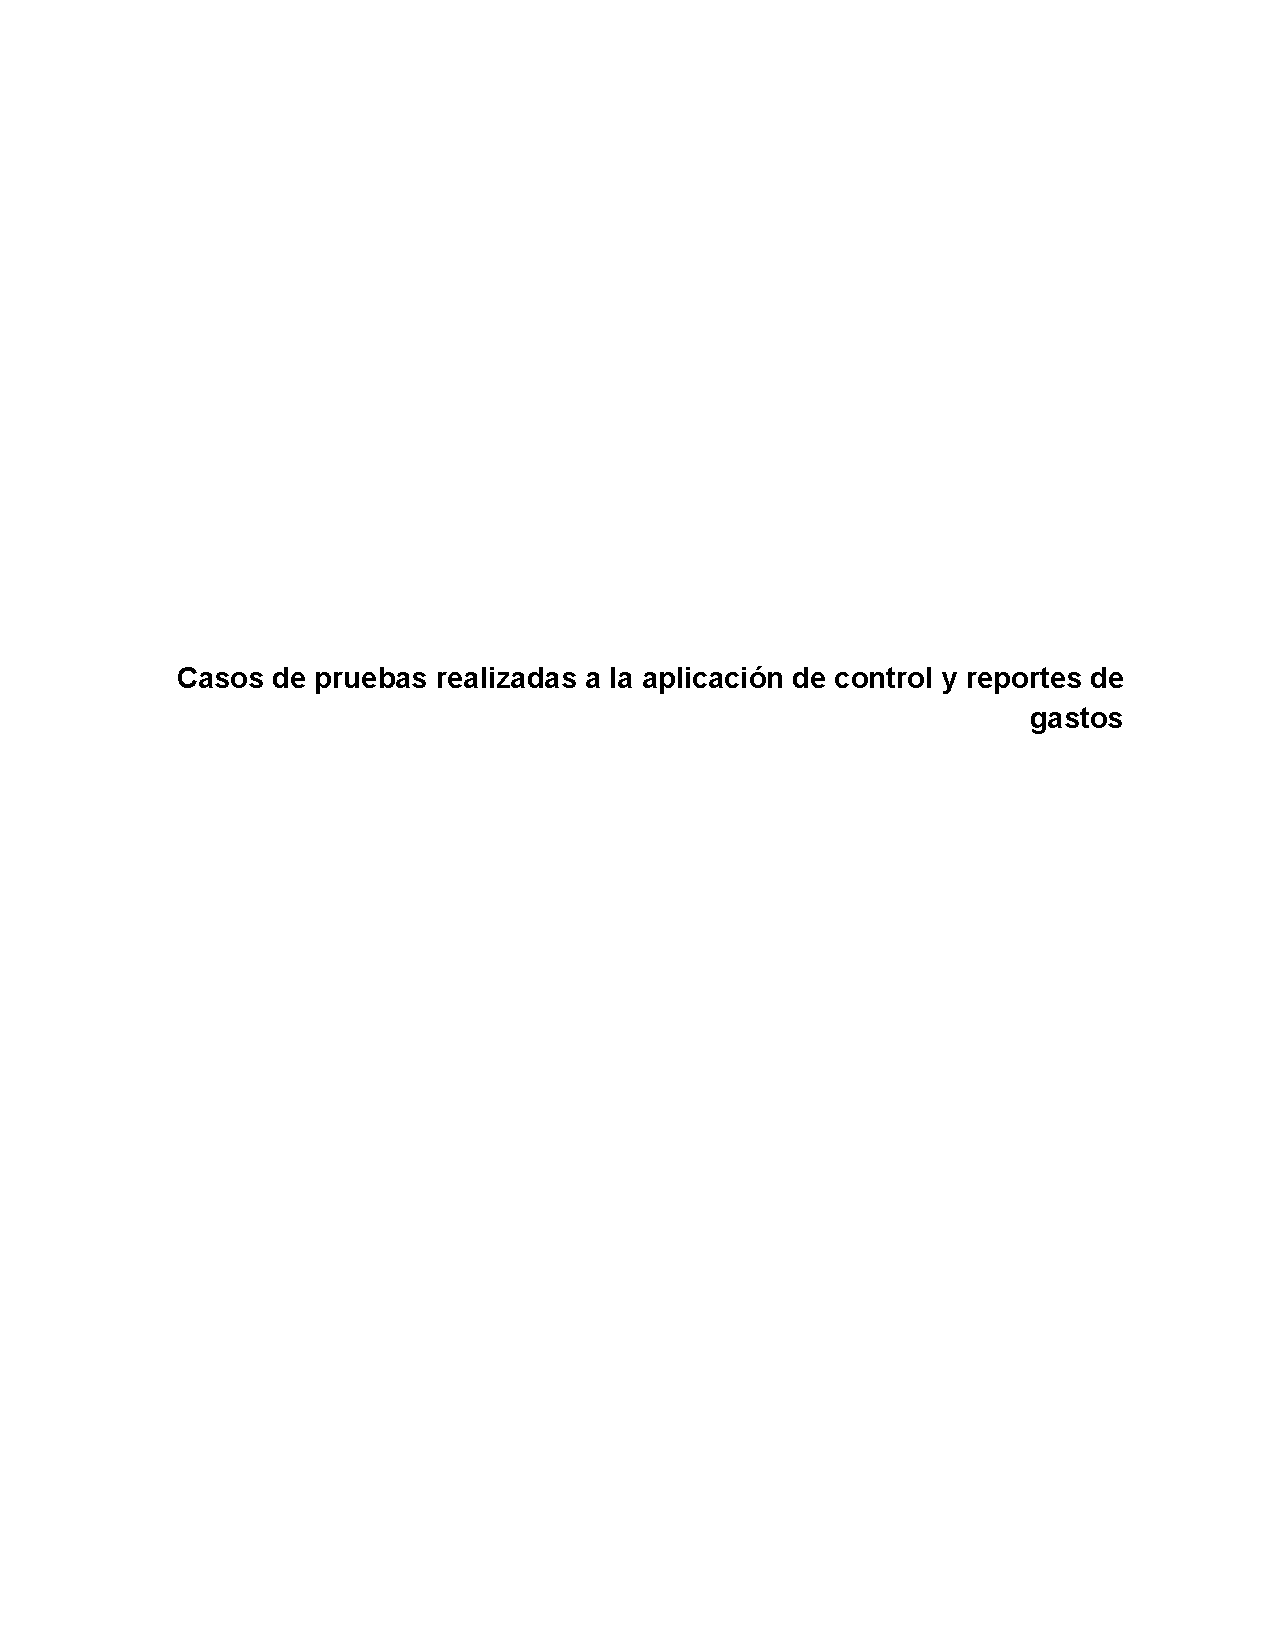
\includepdf[pages=-]{apendices/pruebas.pdf}

\printglossary

\end{document}
